\documentclass[doctor,korean,final]{kmu}

\usepackage{times}
\usepackage{CJKutf8}
\usepackage{mathrsfs}
\usepackage{textcomp}
\usepackage{verbatim}
\usepackage{amsmath}
\usepackage{amsfonts}
\usepackage{xspace}
\usepackage{xcolor}
\usepackage{url}
\usepackage{balance}
\usepackage{booktabs}
\usepackage{multirow}
\usepackage{rotating}
\usepackage{fancyvrb}
\usepackage{lastpage}
\usepackage{alltt}
\usepackage{etoolbox}
\usepackage{cleveref} % After hyperref, listings
\usepackage{fancyhdr}
\usepackage{listings}

\usepackage{macro}
\newenvironment{CompactItemize}{\begin{itemize}}{\end{itemize}}
\def\code#1{{\texttt{#1}}}


\usepackage{caption}
\usepackage{subcaption}

\usepackage{tikz}
\usetikzlibrary{shapes,snakes}


\usepackage{amsmath}
\usepackage{amssymb}
\usepackage{wasysym}

%The given symbol or text (\text{mytext}) in a circle
%To be used always in math mode
\newcommand{\circlesign}[1]{ 
    \mathbin{
        \mathchoice
        {\buildcirclesign{\displaystyle}{#1}}
        {\buildcirclesign{\textstyle}{#1}}
        {\buildcirclesign{\scriptstyle}{#1}}
        {\buildcirclesign{\scriptscriptstyle}{#1}}
    } 
}


\newcommand\buildcirclesign[2]{%
    \begin{tikzpicture}[baseline=(X.base), inner sep=0, outer sep=0]
    \node[draw,circle] (X)  {\ensuremath{#1 #2}};
    \end{tikzpicture}%
}

\definecolor{lbcolor}{rgb}{0.9,0.9,0.9}
\lstset{
    tabsize=2,    
    language=C,
    basicstyle=\footnotesize\ttfamily,
    upquote=true,
    aboveskip={1.5\baselineskip},
    columns=fixed,
    extendedchars=false,
    showtabs=false,
    showspaces=false,
    showstringspaces=false,
    identifierstyle=\ttfamily,
    keywordstyle=\color[rgb]{0,0,1},
    commentstyle=\color[rgb]{0.026,0.112,0.095},
    stringstyle=\color[rgb]{0.627,0.126,0.941},
    numberstyle=\color[rgb]{0.205, 0.142, 0.73},
}


\usepackage{colorhist}
 
\usepackage{minted}
\usepackage{pdfpages}

% 본문 시작
\begin{document}

% 표목차 (List of Tables) 생성
%\listoftables

% 그림목차 (List of Figures) 생성
%\listoffigures

% 위의 세 종류의 목차는 한꺼번에 다음 명령으로 생성할 수도 있습니다.
%\makecontents
%% 한글로 쓴 논문에는 본문에 영문 글자를 쓰지 않는다. 다만, 꼭 필요할 때에는 ‘한글 낱말 (영문 낱말)’ 꼴로 적는다.
%% 이하의 본문은 LaTeX 표준 클래스 report 양식에 준하여 작성하시면 됩니다.
%% 하지만 part는 사용하지 못하도록 제거하였으므로, chapter가 문서 내의
%% 최상위 분류 단위가 됩니다.
%% You cannot use 'part'

%본문을 한글로 작성할 때 머릿말로 시작을 하시는 게 좋습니다. \cite{FD1}
%인용은 다음과 같이 합니다 \cite{RVP1}-\cite{ML2}.
%인용은 뒤에 인용을 쓰는 칸이 있습니다. 참고하여서 인용하시길 바랍니다 \cite{SOCA2,EF2}.
%한글 논문에는 영어를 쓰지 마시기 바랍니다. 

\newif\ifkor
\kortrue 

\includepdf[pages=1-2]{thesis_title.pdf}

% 목차 (Table of Contents) 생성
\tableofcontents
% 그림목차 (List of Figures) 생성
\listoffigures
% 표목차 (List of Tables) 생성
%\listoftables

\pagenumbering{roman}                         % roman 페이지번호로 복원
\setcounter{page}{\value{pagemarker}}         % pagemarker에 저장된 값으로
\addcontentsline{toc}{content}{요약}% 목차(TOC)에 추가
\label{paperlastromanpagelabel}     % <-- 추가 부분: 마지막 페이지 위치 지정

\hfill \break

\newpage \setcounter{pagemarker}{\value{page}}% pagemarker에 다시 저장
\pagenumbering{arabic}                        % arabic 페이지번호로 재시작

\chapter{서론}
\section{서론} \label{sec:introduction}

%$$$$$$$$$$$$$$$$$$$$$$$$$$$$$$$$$$$$$$$$$$$$$$$$$$$$$$$$$$$$$$$$$$$$$$$$$$$$$$$$
%$$$$$$$$$$$$$$$$$$$$$$$$$$$$$$$$$$$$$$$$$$$$$$$$$$$$$$$$$$$$$$$$$$$$$$$$$$$$$$$$
%Background
%$$$$$$$$$$$$$$$$$$$$$$$$$$$$$$$$$$$$$$$$$$$$$$$$$$$$$$$$$$$$$$$$$$$$$$$$$$$$$$$$
최근 코어수가 증가하고 있다. 따라서 멀티코어에서 매니코어 시스템으로 바뀌고 있다. 
매니코어 시스템에 대한 운영체제 커널의 parallelism은 시스템 전체의 parallelism에서 가장 중요하다. 
만약 커널이 scale하지 않으면, 그 위에 동작하는 응용프로그램들도 역시 scale하지 않는다[].
이처럼 중요한 운영체제 커널 중 멀티코어 또는 매니코어 환경에서 많이 사용되는 운영체제가 리눅스 커널이다[].
하지만 리눅스 커널은 아직 확장성 문제가
있다~\cite{SilasBoydWickizer2010LinuxScales48}~\cite{Changwoo2016UMSF}.
확장성 문제 중 하나는 락 경합 때문에 발생하는 업데이트 직렬화
문제이다~\cite{Matveev2015RLU}~\cite{Dodds2015SCT}.
그 이유는 업데이트 오퍼레이션은 여러 쓰레드가 동시에 수행되지 못하기
때문이다~\cite{mckenney2011parallel}.

이처럼 업데이트 직렬화 문제를 해결하기 위해 여러 동시적 업데이트 방법 들이 연구되고
있다~\cite{Arbel2014ConcurrentRCU}~\cite{Matveev2015RLU}.
이러한 동시적 업데이트 방법들은 워크로드 특성인 업데이트 비율에 따라 많은 성능 차이를
보인다~\cite{Matveev2015RLU}.
이 중 높은 업데이트 비율을 가진 자료 구조 때문에 발생하는 학장성 문제를 해결하기 위한 여러 방법이 연구 되고
있다.
그 중 하나는 cache communication bottleneck을 줄인 log-based
알고리즘~\cite{Shalev2006PLS}~\cite{Hendler2010FC}~\cite{SilasBoydWickizerPth}을
사용하는 것이다.
Log-based 알고리즘은 업데이트가 발생하면, data structure의 업데이트 operation을
per-core 또는 atomic하게 log로 저장하고 read operation을 수행하기 전에 저장된 로그를 수행하는것이다 .
이것은 마치 CoW(Copy On Write)와 유사하다~\cite{PaulDetailLWN}.

S. Boyd-Wickizer et al.는 동기화된 타임스탬프 카운터(synchronized timestamp counters) 기반의
per-core log를 활용하여 update-heavy한 자료구조를 대상으로 동시적 업데이트 문제를
해결함과 동시에 cache communication bottleneck을 줄였다~\cite{SilasBoydWickizerPth}.
동기화된 타임스탬프 카운터 기반의 per-core log를 활용한 동시적 업데이트방법은
업데이트 부분만 고려했을 때, per-core에 데이터를 저장함으로 굉장히 높은 scalability를 가진다[].
하지만 per-core 기반의 동기화된 타임스탬프 카운터를 사용한 방법은 결국 timestamp merging and ordering 작업을
야기한다.
만약 코어 수가 늘어 날 경우, 로그를 자료 구조에 적용하는 과정에서 timestamp 때문에 발생하는 추가적인 sequntial 프로세싱이
요구된다.
이것은 결국 확장성과 성능을 저해한다. 

본 논문은 동기화된 타임스탬프 카운터를 이용함에 따라 생기는 추가적인 sequencial processing 문제를
해결하기 위해 LDU(Lightweitgh log-based Deferred Update)를 개발하였다. 
LDU는 타임스탬프 카운터가 필요한 operation log를 업데이트 순간마다 지우고, 매번 로그를 생성하지 않고 재활용하는 방법이다.
이로인해 synchronized timestamp counter 문제와 cache communication bottleneck 문제를 동시에
해결하였다.
해결 방법은 분산 시스템에서 사용하는 log기반의 concurrent updates 방식과 shared-memory system의 
hardware-based synchronization 기법(compare and swap, test and
set, atomic swap)을 조합하여 동시적 업데이트 문제를 해결하였다.

이처럼 동기화된 타임스탬프 카운터를 제거함과 동시에, cache communication bottleneck 줄인
LDU는 log-based 알고리즘들의 장점들을 모두 포함할 뿐만아니라 추가적인 장점을 가진다.
첫째로, update가 수행하는 시점 즉 로그를 저장하는 순간에는 lock이 필요가 없다. 
따라서 lock에 대한 오버헤드 없이 concurrent updates를 수행할 수 있다
둘째로, 저장된 update operation log를 coarse-grained lock과 함께 하나의 코어에서 수행하기 때문에,
cache 효율성이 높아진다~\cite{Hendler2010FC}.
셋째로, 기존 여러 자료구조에 쉽게 적용할 수 있는 장점이 있다.
게다가 마지막으로, log를 저장하기 전에 로그를 삭제하므로 보다 빠르게 log의 수를 줄일 수 있다. 

우리는 위와 같은 장점을 가지는 LDU를 리눅스 커널에서 high update rate 때문에 scalability 문제를 야기시키는
anonymous reverse mapping과 file reverse mapping에 적용하였다.
또한 우리는 LDU를 Linux 4.5.rc4에 구현하였고, fork-intensive 워크로드인
AIM7~\cite{AIM7Benchmark}, Exim~\cite{Exim} from MOSBENCH~\cite{MOSBENCH},
lmbench~\cite{mcvoy1996lmbench}를 대상으로 성능 개선을 보였다. 개선은 stock 리눅스 커널에 비해 120코어에서
각각 x,x,x 배이다.

\noindent
\textbf{Contributions.} This paper makes the following contributions:
\begin{itemize}
\item 우리는 리눅스 커널을 위한 새로운 log-based concurrnet updates 방법인 LDU를 개발하였다. 
LDU는 동기화된 타임스탬프 카운터를 이용함에 따라 생기는 시간 정렬과 머징에 의한 추가적인 sequencial processing 문제를
해결하였다.
이를 위해 LDU는 로그를 업데이트 순간 지우고 로그를 재활용하는 방법을 개발하였다. 
\item 우리는 LDU을 practical한 manycore system인 intel xeon 120코어 위에 동작하는 리눅스 커널의
2가지 reverse mapping(anonymous, file)에 적용하여, fork scalability 문제를 해결하였다.
Fork 관련 벤치마크 성능은 워크로드 특성에 따라 1.6x부터 2.2x까지 개선되었다.
\end{itemize}

The rest of this paper is organized as follows.
Section 2 describes the background and Linux scalability problem.
Section 3 describes the design of the LDU algorithm and 
Section 4 explains how to apply to Linux kernel.
section 5 explains our implementations in Linux and
Section 6 shows the results of the experimental evaluation. 
Finally, section 8 concludes the paper.


%$$$$$$$$$$$$$$$$$$$$$$$$$$$$$$$$$$$$$$$$$$$$$$$$$$$$$$$$$$$$$$$$$$$$$$$$$$$$$$$$
%$$$$$$$$$$$$$$$$$$$$$$$$$$$$$$$$$$$$$$$$$$$$$$$$$$$$$$$$$$$$$$$$$$$$$$$$$$$$$$$$
%Method
%$$$$$$$$$$$$$$$$$$$$$$$$$$$$$$$$$$$$$$$$$$$$$$$$$$$$$$$$$$$$$$$$$$$$$$$$$$$$$$$$
`



%$$$$$$$$$$$$$$$$$$$$$$$$$$$$$$$$$$$$$$$$$$$$$$$$$$$$$$$$$$$$$$$$$$$$$$$$$$$$$$$$
%$$$$$$$$$$$$$$$$$$$$$$$$$$$$$$$$$$$$$$$$$$$$$$$$$$$$$$$$$$$$$$$$$$$$$$$$$$$$$$$$
%Mapping
%$$$$$$$$$$$$$$$$$$$$$$$$$$$$$$$$$$$$$$$$$$$$$$$$$$$$$$$$$$$$$$$$$$$$$$$$$$$$$$$$






%$$$$$$$$$$$$$$$$$$$$$$$$$$$$$$$$$$$$$$$$$$$$$$$$$$$$$$$$$$$$$$$$$$$$$$$$$$$$$$$$
% Reference Sentence 1
%$$$$$$$$$$$$$$$$$$$$$$$$$$$$$$$$$$$$$$$$$$$$$$$$$$$$$$$$$$$$$$$$$$$$$$$$$$$$$$$$






%$$$$$$$$$$$$$$$$$$$$$$$$$$$$$$$$$$$$$$$$$$$$$$$$$$$$$$$$$$$$$$$$$$$$$$$$$$$$$$$$
%Reference Sentence 2:LDU paper
%$$$$$$$$$$$$$$$$$$$$$$$$$$$$$$$$$$$$$$$$$$$$$$$$$$$$$$$$$$$$$$$$$$$$$$$$$$$$$$$$
% Ondemand로 로그를 지워 준다.
%Background
%With the drastic increase of CPU core counts in various high-end
%server systems, achieving performance scalability of operating systems
%running on such many-core systems has been an important issue in research
%communities.
%Linux has been naturally considered as a major target for the scalability
%improvement and a number of accomplishments are published.
%Early results include RCU~\cite{McKenney98} and hazard
%pointer~\cite{MagedMichael04a} to improve scalability for read-most data 
%structures in the Linux kernel. %for relatively low CPU core counts.
%Though the early results show certain level of improvement in scalability,
%it turned out that more significant portion of scalability limitation of
%Linux kernel is due to lock contention in update-heavy global data structures 
%including file reverse mappings and anonymous reverse mappings during
%spawning child processes~\cite{Andi2011adding}~\cite{Tim2013adding}. 
%Such update-heavy data structures cause serialization of the update operations
%leading to severe performance degradation. 

%Scaling operating systems to many-core architectures is one of the most
%important challenges in computing today. 
%One of the scalable operations system is Linux because the Linux kernel
%community has made it scalable.
%For example, read-mostly data structures in the Linux have been achieved
%considerable multi-core scaling by using RCU~\cite{McKenney98} and hazard
%pointer~\cite{MagedMichael04a}.
%However, the Linux kernel suffers from such scalability bottlenecks at high
%core counts.
%The Linux kernel on many-core processors can be
%bottlenecked by contended updates locks where processes share a global data
%structure.
%When a process spawns child process, reverse mapping using shared global
%data structure suffers from updates lock contention.
%Recent research shows how to run a fork in parallel with creating new reverse
%mapping data structure~\cite{SilasBoydWickizerPth}.
%More specifically, in order to perfect scalability of the fork, both the
%file reverse mapping and the anonymous reverse mapping can execute
%update concurrently without lock
%contention~\cite{Andi2011adding}~\cite{Tim2013adding}.

%The fundamental scalability problem of reverse mapping is their serialized
%update because operating systems are serialized at the update operation.

%To solve this problem, an existing approach is to make the update-heavy data
%structures as non-blocking~\cite{Harris2001Lockfree} based on
% \emph{compare-and-swap}(CAS).
%Introducing non-blocking data structures eliminates the update serialization
% problem during process spawning, but incurs additional issues due to
% inter-core communication
%bottlenecks and cache coherence system's write
% serialization~\cite{SilasBoydWickizerPth}.
%To overcome the issues caused by cache coherence system, S. Boyd-Wickizer et
% al. proposed Oplog~\cite{SilasBoydWickizerPth} where logs update operations
% with time stamps and actual updates are performed later when the updated data
% need to be read.
%While Oplog nicely solves the update serialization problem without any cache
% coherence-related overheads, the merging of the update logs recorded in
% multiple per-core data structures considering time stamps further causes
% performance overheads resulting in limited scalability
% improvement~\cite{McKenney2008ParallelProgramming}.

%Therefore, many researches have proposed non-blocking
%algorithms~\cite{Harris2001Lockfree} for concurrent data structure based on
%\emph{compare-and-swap}(CAS);nonetheless, this method may suffer from inter-core
%communication bottleneck, the cache coherence system serializes the
% writes~\cite{SilasBoydWickizerPth}.

%Another a existing solution is using the per-core processing like
%Oplog~\cite{SilasBoydWickizerPth}, which achieves scalability by logging in
%per-core memory.
%In fact, per-core approach may have best performance for the update-heavy data
%structure because of their partitioned data structures, whose updates can
%operate locally.
%The more-expensive reads, however, must merge across the entire per-core
%data;read operations are expensive~\cite{McKenney2008ParallelProgramming}.
%Therefore, their approach may be complex with regard to the read operation.
%This paper attacks this complexity as a result of the per-core processing.
%Even though they have generalized a per-core processing to the Oplog's library, 
%they use intricate optimizations, so their optimizations may be expensive with
%regard to the read operation.
%For example, they use the absorbing updates that removes the cancelable
%operation before the read.
%This operation may need to iterate previous operation log due to searching the
%cancelable operation log.
%Furthermore, reducing the memory use, they maintain per-core memory space.

%Method
%This paper proposes a novel concurrent update method, \deferu, applicable to
% Linux reverse mapping solving the problems 
%mentioned above: the overheads caused by inter-core communication bottlenecks
% and per-core log management with time stamps. 
%Our goal is to make the Linux fork scale to large numbers of cores using
%lightweight deferred processing algorithm.
%The fork scalability requires two challenges in designing a reverse mapping.
%First, this lightweight method should permit the concurrent updates not only to
%reduce the inter-core communication bottleneck but also to eliminate their 
%complexity.
%Second, this lightweight method should apply to Linux reverse mapping, and
%improve the Linux fork scalability.

%The \deferu is similar to Oplog in that it defers the actual update operations
% as late as possible to reduce serialization problems, but it uses a light
% weight global queue with non-blocking synchronization for update logs and
% eliminates time stamps required for per-core log management. 
%In addition, to optimize the log management and minimize the traversal
% overheads during reading, \deferu applies update-side absorbing algorithm based on atomic
%marking and thus efficiently find the operations to be canceled. 
%The evaluation of the proposed \deferu on Linux kernel 3.19.rc4 running on a
% 120 core system reveals that 
%the execution times could be improved by 1.7x, 1.6x, and 2.2x for 
%a fork-intensive workload-
%AIM7~\cite{AIM7Benchmark}, Exim from
%MOSBENCH~\cite{SilasBoydWickizer2010LinuxScales48}, and 
%lmbench~\cite{mcvoy1996lmbench}, respectively.

%Second, it uses a novel update-side absorbing that uses the atomic marking
%method, which allows \deferu to eliminate read-side traversal for finding the
%cancelable operation log;readers can improve performance.

%The proposed approach has the following advantages. 
%First, it can permits the reverse mapping to remove lock contention, so Linux's
%fork scalability has been improved.
%Second, using the lightweight update-side absorbing, \deferu can reduce
%complexity and improve readers performance.
%Finally, while per-core processing uses the time-stamp counter(e.g., RDTSCP,
%RDTSC) that depend on hardware, our method may not depend on hardware.

%We implemented the \deferu in a Linux 3.19.rc4 with modification of lock. 
%We evaluated the performance and scalability using a fork-intensive workload-
%AIM7~\cite{AIM7Benchmark}, Exim from
%MOSBENCH~\cite{SilasBoydWickizer2010LinuxScales48},
%lmbench~\cite{mcvoy1996lmbench}-our design improves throughput and execution
%time on 120 core by 1.7x, 1.6x, 2.2x respectively, relative to stock Linux.

%Mapping
%Paragraph 
%This paper is organized as follows. 
%Section 2 summarizes related works and compare our contributions to previous
%works. 
%Section 3 describes the design of the \deferu algorithm and 
%Section 4 explains how to apply to Linux kernel.
%section 5 explains our implementations in Linux and
%Section 6 shows the results of the experimental evaluation. 
%Finally, section 7 concludes the paper.

\chapter{연구 배경 및 관련 연구}\label{sec:related}
\section{Related work} \label{sec:RelatedWork}
%$$$$$$$$$$$$$$$$$$$$$$$$$$$$$$$$$$$$$$$$$$$$$$$$$$$$$$$$$$$$$$$$$$$$$$$$$$$$$$$$
%Paragraph 1:Linux Scalability의 연구에 대한 설명
%$$$$$$$$$$$$$$$$$$$$$$$$$$$$$$$$$$$$$$$$$$$$$$$$$$$$$$$$$$$$$$$$$$$$$$$$$$$$$$$$

\noindent
\textbf{Operating system scalability.}
~\cite{Clements15SCR}In order to improve Linux scalability, researchers have
been optimized memory management in Linux by finding and fixing scalability
bottlenecks~\cite{BoydWickizer2008Corey}~\cite{BoydWickizer2012OLS}.
Shared address spaces in multithreaded applications 
easily become scalability bottlenecks since kernel operations 
including \code{mmap} and \code{munmap} system calls and \code{page faults}
 handling require per-process locks for synchronization.
Multithreaded application, for example, can become bottleneck by kernel
operations on their shared address space, whose operations are the \code{mmap}
and \code{munmap} system calls and \code{page faults}.
These operations are synchronized by a single per-process lock.
BonsaiVM~\cite{AustinTClements2012RCUBalancedTrees} solved this address space
problem by using the RCU;
RadixVM~\cite{Clements2013RadixVM} created a new VM using refcache and radix
tree, which enable \code{munmap}, \code{mmap}, and \code{page fault} on
non-overlapping memory regions to scale perfectly.
Alternatively, to avoid contention caused by shared address space locking,
system programmers change their multithreaded applications to use
processes~\cite{SilasBoydWickizer2010LinuxScales48}.


%$$$$$$$$$$$$$$$$$$$$$$$$$$$$$$$$$$$$$$$$$$$$$$$$$$$$$$$$$$$$$$$$$$$$$$$$$$$$$$$$
%Paragraph 2:Concurrent updates에 대한 연구
%$$$$$$$$$$$$$$$$$$$$$$$$$$$$$$$$$$$$$$$$$$$$$$$$$$$$$$$$$$$$$$$$$$$$$$$$$$$$$$$$
\noindent
\textbf{Scalabe data structure.}
~\cite{Dodds2015SCT}Though sufficient level of performance scalability has been
achieved for reader intensive operations through RCU and Hazard pointer, 
solutions to scalability for update-heavy operations has not been satisfiable.
A recent paper by Arbel and Attiya~\cite{Arbel2014ConcurrentRCU} shows a new
design of concurrent search tree called the Citrus tree. The Citrus tree
combines RCU and fine-grained locks, and it supports concurrent write
operations that traverse the search tree by using RCU concurrently.
When increasing the update rate, Citrus tree still suffers from bottlenecks.
RLU~\cite{Matveev2015RLU} presents a new synchronization mechanism that allows
unsynchronized sequences of reads to execute concurrently with updates.
In high update rate, Oplog can achieve substantially multi-core scaling for
update-heavy data structures.
Our work focus on update-heavy data structures and uses non-blocking method to
 store the operation log instead of per-core processing.


%$$$$$$$$$$$$$$$$$$$$$$$$$$$$$$$$$$$$$$$$$$$$$$$$$$$$$$$$$$$$$$$$$$$$$$$$$$$$$$$$
%Paragraph 3: Scalable Data Structure and Lock에 대한 연구
%$$$$$$$$$$$$$$$$$$$$$$$$$$$$$$$$$$$$$$$$$$$$$$$$$$$$$$$$$$$$$$$$$$$$$$$$$$$$$$$$
\noindent
\textbf{Scalable lock.}
~\cite{Wang2016BeMyGuest}~\cite{Bueso2015STP}~\cite{Bueso2014MCS}One method for
the concurrent update is using the non-blocking algorithms~\cite{Harris2001Lockfree}~\cite{Fomitchev2004Lockfree}~\cite{Timnat2012},
 which are based on CAS.


MCS~\cite{MellorCrummey91}, a scalable exclusive lock, is used in the Linux
kernel~\cite{MCSLocksKernel}.
to avoid unfairness at high contention levels, so this scalable exclusive
lock can be used for fine grained locking in Linux. 
However, in MCS, since only one thread may hold the lock at a time, it can
cause low scalability in case of long critical regions.
Reader-writer lock~\cite{Courtois71} allows either number of readers to execute
concurrently or single writer to execute.
Thus, readers-writer locks allow better scalability in case of read-mostly 
objects.

In read-mostly data structures, RCU~\cite{McKenney98} can be quite useful
since it allows read operations to proceed without read locks, and delays
freeing of data structures to avoid races. One drawback is that as the update
rate increases, their performance and scalability decrease due to a single
writer and their synchronization function.
Consequently, 
scalable exclusive lock, reader-writer lock
and RCU require serialization for updates and thus show significant limitation
 on scalability. 



%$$$$$$$$$$$$$$$$$$$$$$$$$$$$$$$$$$$$$$$$$$$$$$$$$$$$$$$$$$$$$$$$$$$$$$$$$$$$$$$$
%$$$$$$$$$$$$$$$$$$$$$$$$$$$$$$$$$$$$$$$$$$$$$$$$$$$$$$$$$$$$$$$$$$$$$$$$$$$$$$$$
%Reference Sentence 1
%$$$$$$$$$$$$$$$$$$$$$$$$$$$$$$$$$$$$$$$$$$$$$$$$$$$$$$$$$$$$$$$$$$$$$$$$$$$$$$$$




%$$$$$$$$$$$$$$$$$$$$$$$$$$$$$$$$$$$$$$$$$$$$$$$$$$$$$$$$$$$$$$$$$$$$$$$$$$$$$$$$
%Reference Sentence 2:LDU paper
%$$$$$$$$$$$$$$$$$$$$$$$$$$$$$$$$$$$$$$$$$$$$$$$$$$$$$$$$$$$$$$$$$$$$$$$$$$$$$$$$

%Paragraph 1:Linux Scalability의 연구에 대한 설명
%In order to improve Linux scalability, researchers have been optimized memory
%management in Linux by finding and fixing scalability bottlenecks.

%Shared address spaces in multithreaded applications 
%easily become scalability bottlenecks since kernel operations 
%including \code{mmap} and \code{munmap} system calls and \code{page faults}
% handling require per-process locks for synchronization.
%Multithreaded application, for example, can become bottleneck by kernel
%operations on their shared address space, whose operations are the \code{mmap}
%and \code{munmap} system calls and \code{page faults}.
%These operations are synchronized by a single per-process lock.
%BonsaiVM~\cite{AustinTClements2012RCUBalancedTrees} solved this address space
%problem by using the RCU;
%RadixVM~\cite{Clements2013RadixVM} created a new VM using refcache and radix
%tree, which enable \code{munmap}, \code{mmap}, and \code{page fault} on
%non-overlapping memory regions to scale perfectly.
%Alternatively, to avoid contention caused by shared address space locking,
%system programmers change their multithreaded applications to use
%processes~\cite{SilasBoydWickizer2010LinuxScales48}.
 
%Paragraph 2:Fork Scalability에 대한 설명
%Multi-processing environment 
%suffers from scalability bottlenecks due to the well-known fork
%scalability problem~\cite{Andi2011adding}~\cite{Tim2013adding}.
%When Linux spawns child process, the Linux substantially performs locks because
%of protecting the reverse mapping data structure naturally causing
%bottlenecks.
%Oplog~\cite{SilasBoydWickizerPth}, which is an important basis of our approach,
%solves this problem using time-stamp log and
%per-core processing.


%\subsection{Locking}
%Paragraph 1: Locks에 대한 설명
%MCS~\cite{MellorCrummey91}, a scalable exclusive lock, is used in the Linux
%kernel~\cite{MCSLocksKernel}.
%to avoid unfairness at high contention levels, so this scalable exclusive
%lock can be used for fine grained locking in Linux. 
%However, in MCS, since only one thread may hold the lock at a time, it can
%cause low scalability in case of long critical regions.
%Reader-writer lock~\cite{Courtois71} allows either number of readers to execute
%concurrently or single writer to execute.
%Thus, readers-writer locks allow better scalability in case of read-mostly 
%objects.

%In read-mostly data structures, RCU~\cite{McKenney98} can be quite useful
%since it allows read operations to proceed without read locks, and delays
%freeing of data structures to avoid races. One drawback is that as the update
%rate increases, their performance and scalability decrease due to a single
%writer and their synchronization function.
%Consequently, 
%scalable exclusive lock, reader-writer lock
%and RCU require serialization for updates and thus show significant limitation
% on scalability. 

%\subsection{Non-Blocking algorithm}

%Paragraph 1: Lock-free 방법 설명
%One method for the concurrent update is using the non-blocking
%algorithms~\cite{Harris2001Lockfree}~\cite{Fomitchev2004Lockfree}~\cite{Timnat2012},
% which are based on CAS.
%In non-blocking algorithms, each core tries to read the values of shared
%data structures from its local location, but has possibility of reading 
%obsolete values.
%CAS is performed at the time of reading values that are not the current values
%and CAS fails and requires retrials sometimes when the values have been
% overwritten.
%These algorithms execute optimistically as though they read the value at
%location in their data structure;they may obtain stale data at the time.
%When they observed against the current value, they execute a CAS to compare the
%against value.
%The CAS fails when the value has been overridden, and they must be
%retried later on.
%Consequently, both repeated CAS operation and their iteration loop caused by
%CAS fails cause bottlenecks due to inter-core communication
% overheads~\cite{SilasBoydWickizerPth}.
%Moreover, none of the non-blocking algorithms implements an iterator, whose
%data structure just consists of the insert, delete and contains
%operations~\cite{petrank2013lock}.
%The Linux, however, commonly uses the iteration to read, so when applying
%non-blocking algorithms to the Linux, they may meet this iteration problem.
%Petrank~\cite{petrank2013lock} solved this problem by using a consistent
%snapshot of the data structure; this method, however, may require a lot of
%effort to apply its sophisticated algorithms to Linux.
%For evaluation purposes, we implemented Harris linked
%list~\cite{Harris2001Lockfree} to Linux, and we sometimes have failure where
%reading the pointer that had been deleted by updater concurrently result of the
%problem of the iteration.

%Paragraph 2: Linux llist 설명
%Linux kernel uses lock-less list("lock-less NULL terminated single
%list") that are widely used in the Linux kernel to improve scalability.
%In order to delete operation for multiple consumer, the existing
%algorithms traverse the list from beginning or their optimized point.
%On the other hand, lock-less list inserts node at the first of the list, so
% when the CAS operation fails, they will minimally traverse from the head
% node.
%Although lock-less list uses a non blocking method, they retries minimally
%and thus they can significantly reduce inter-core communication bottleneck and
% the repeated loop bottleneck.
%Our proposed method uses this feature in case of inserting the operation log.

%\subsection{Concurrent Update}
%Paragraph 1: Update Rate
%Though sufficient level of performance scalability has been achieved for 
%reader intensive operations through RCU and Hazard pointer, 
%solutions to scalability for update-heavy operations has not been satisfiable.
%A recent paper by Arbel and Attiya~\cite{Arbel2014ConcurrentRCU} shows a new
%design of concurrent search tree called the Citrus tree. The Citrus tree
%combines RCU and fine-grained locks, and it supports concurrent write
%operations that traverse the search tree by using RCU concurrently.
%When increasing the update rate, Citrus tree still suffers from bottlenecks.
%RLU~\cite{Matveev2015RLU} presents a new synchronization mechanism that allows
%unsynchronized sequences of reads to execute concurrently with updates.
%In high update rate, Oplog can achieve substantially multi-core scaling for
%update-heavy data structures.
%Our work focus on update-heavy data structures and uses non-blocking method to
% store the operation log instead of per-core processing.

\chapter{논문에서 해결하고자 하는 구체적인 문제}\label{sec:problem}
\section{Background and Problem}\label{sec:bg}

%$$$$$$$$$$$$$$$$$$$$$$$$$$$$$$$$$$$$$$$$$$$$$$$$$$$$$$$$$$$$$$$$$$$$$$$$$$$$$$$$
% Paragraph : Linux Scalability : Fork intensive workload 문제점 설명 
%$$$$$$$$$$$$$$$$$$$$$$$$$$$$$$$$$$$$$$$$$$$$$$$$$$$$$$$$$$$$$$$$$$$$$$$$$$$$$$$$

\begin{figure}[h]
  \begin{subfigure}{0.45\textwidth}
    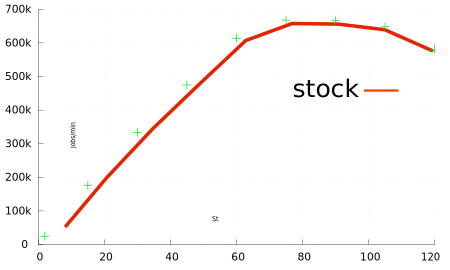
\includegraphics[width=\textwidth]{graph/aim7_default}
    \caption{AIM7-multiuser scalability}
  \end{subfigure}%
  \begin{subfigure}{0.45\textwidth}
    \includegraphics[width=\textwidth]{graph/lockstat}
    \caption{Lock wait time on 120 core}
  \end{subfigure}
  \centering
  \caption{Scalability of AIM7 multiuser and wait time to acquire locks on 120 core.
  This workload simultaneously create many processes. The (a) shows up to 75
  core, the stock Linux scales linearly, then it flattens out. The (b) left bar 
  represents anonymous reader-writer semaphore causes a scalability bottleneck, 
  and The (b) right bar shows file mapping reader-writer semaphore causes a
  scalability bottleneck.}
  \label{fig:aim7_default}
\end{figure}

Applications' performance would be limited by the operating system kernel when 
the operating system kernel does not scale well~\cite{Clements15SCR}~\cite{Boyd-WickizerCorey}.
%Linux has heavily optimized for multi-core operating systems.
To analyze the current status of the operating system scalability,
we measured the performance trends of the AIM7-multiuser benchmark on Linux
with various CPU cores.
The AIM benchmark has, until recently, been widely used in research area
and the Linux community~\cite{Bueso2015STP}~\cite{Bueso2014MCS}.
The AIM7-multiuser workload simultaneously creates many processes with
disk-file operations, virtual memory operations, pipe I/O, and arithmetic
operations.
%We used the temp filesystem to minimize the filesystem bottlenecks.
The result of figure~\ref{fig:aim7_default}(a) shows that
Linux shows significantly limited performance scalability when CPU core 
exceeds 75.

%$$$$$$$$$$$$$$$$$$$$$$$$$$$$$$$$$$$$$$$$$$$$$$$$$$$$$$$$$$$$$$$$$$$$$$$$$$$$$$$$
% Paragraph: Lockstat로 분석 결과 설명 
%$$$$$$$$$$$$$$$$$$$$$$$$$$$$$$$$$$$$$$$$$$$$$$$$$$$$$$$$$$$$$$$$$$$$$$$$$$$$$$$$

To understand the sources of scalability bottleneck on 120 core systems, we profiled a 
lock contention using the \code{lock\_stat}~\cite{LOCKSTAT}, a Linux kernel lock profiler that reports how
long each lock is held and the wait time to acquire the lock.
The figure~\ref{fig:aim7_default}(b) shows the cost of acquiring the lock for the AIM7-multiuser
running on a 120 core system.
Results of the \code{lock\_stat} that the main source of lock contention was the 
anonymous reverse mapping semaphore(\code{anon\_vma->rwsem}), 
which was caused by simultaneously creating a number of processes.
%The reverse page mapping records page information when using fork(), exit() and
%mmap() system call to find all page table entries.
To understand further bottlenecks, we intentionally removed the kernel codes causing 
anonymous reverse mapping which has been revealed as the most significant source of the problem.
%conducted a workaround by removing
%anonymous reverse mapping relative code in the part of the Linux fork with page-swap off
%because of avoiding the Linux page reclaiming.
When the anonymous reverse mapping code was removed, 
the second major source of the bottleneck was file 
reverse mapping reader-writer semaphore(\code{mapping->i\_mmap\_rwsem}).

%$$$$$$$$$$$$$$$$$$$$$$$$$$$$$$$$$$$$$$$$$$$$$$$$$$$$$$$$$$$$$$$$$$$$$$$$$$$$$$$$
% Paragraph : 리눅스 reverse page map의 write serialization 문제점
%$$$$$$$$$$$$$$$$$$$$$$$$$$$$$$$$$$$$$$$$$$$$$$$$$$$$$$$$$$$$$$$$$$$$$$$$$$$$$$$$

Our background study showed that both the anonymous reverse mapping
reported from the Linux community~\cite{Andi2011adding} and the file reverse mapping reported from S.
Boyd-Wickizer~\cite{SilasBoydWickizerPth} are significant factors in fork scalability problem.
Thus, in order to perfect scalability of the fork, both the
file reverse mapping and the anonymous reverse mapping should be executed
concurrently without any lock.
%In fact, the fundamental scalability problem of reverse mapping is their
%serialized update operations because operating systems are serialized at
%the update operations.

%$$$$$$$$$$$$$$$$$$$$$$$$$$$$$$$$$$$$$$$$$$$$$$$$$$$$$$$$$$$$$$$$$$$$$$$$$$$$$$$$
% Paragraph : update heavy한 상황에 대한 설명과 해결 방법에 대한 설명
%$$$$$$$$$$$$$$$$$$$$$$$$$$$$$$$$$$$$$$$$$$$$$$$$$$$$$$$$$$$$$$$$$$$$$$$$$$$$$$$$

Existing research accomplishments to achieve scalable concurrent update in many
core systems are categorized into two methods:
non-blocking
algorithms~\cite{Harris2001Lockfree}~\cite{Fomitchev2004Lockfree}~\cite{Timnat2012}
in early stages and log-based algorithms.
In non-blocking algorithms, update operation observes against the current
value in global data structure, and they execute an atomic compare and swap(CAS) to 
compare the against value.
When the value has been overridden, the updater must be retried.
Consequently, both the repeated global CAS operation and the iteration loop caused
by CAS fails will result in bottlenecks due to inter-core communication
overheads~\cite{SilasBoydWickizerPth}.
To overcome the problem of cache coherence systems, log-based methods are
proposed.
%Our research also uses a log-based deferred design that alows concurrent
%updates to scale, so that multiprocessed applications can scale to large
% numbers of cores.

%$$$$$$$$$$$$$$$$$$$$$$$$$$$$$$$$$$$$$$$$$$$$$$$$$$$$$$$$$$$$$$$$$$$$$$$$$$$$$$$$
%Paragraph : Log 기반의 알고리즘 대략적인 설명 
%$$$$$$$$$$$$$$$$$$$$$$$$$$$$$$$$$$$$$$$$$$$$$$$$$$$$$$$$$$$$$$$$$$$$$$$$$$$$$$$$

%Log-based algorithm is that when update operations occur, it logs the update
%operation and applies the all operation logs to the data structure
%before read operation, so reader can read up to date data structure.

The log-based algorithms are
a suitable solution for the update-heavy data structure because they allow
update operations to proceed with a coarse-grained update lock or without
update locks.
The benefit of avoiding a fine-grained update lock can eliminate the overhead of
acquiring a lock that requires fetching the lock's cache line.
Thus, it reduces the cache communication traffic;a contended cache line on
many-core processors can take hundreds of cycles to fetch from a remote
core~\cite{AustinTClements2012RCUBalancedTrees}, and these techniques can be easily applied to other data structures.
%In addition to avoiding fine-grained lock and easily applying the
%other data structures, a log-based method can remove an existing
%operation log rather than actually executing a operation log.

One notable recent research accomplishment regarding log-based approach is
the OpLog proposed by S. Boyd-Wickizer \textit{et al.}.
The OpLog utilizes representative distributed systems management concepts(e.g., Google spanner's 
synchronized clocks scheme~\cite{Corbett2013SGG}) and proposes the log-based algorithm to shared-memory systems.
The OpLog shows significant improvement in performance scalability for update-heavy operating system
data structures.
Though the OpLog forms an important basis for another step of improvement in performance
scalability problem in many core systems, it still has limitation that it's 
synchronized time-stamp counters might cause additional overhead during log management
process.
%The OpLog using the synchronized time-stamp counters method may incur
%time-stamp merging and ordering process.
%Consequently, when core counts increases, the time-stamp merging and ordering
%process may require sequential processing, which can limit scalability and
%performance.
%For example, if cores counts are 1000 and per-core logs counts are 10, 
%because each log searches all core's log, 
\chapter{로그기반 동시적 업데이트 방법}
\section{LDU Design}

%$$$$$$$$$$$$$$$$$$$$$$$$$$$$$$$$$$$$$$$$$$$$$$$$$$$$$$$$$$$$$$$$$$$$$$$$$$$$$$$$
%Paragraph 1: LDU의 특징을 간단한 설명과 이번장에 대한 설명(LDU의 특징을 요약하여 설명)
%$$$$$$$$$$$$$$$$$$$$$$$$$$$$$$$$$$$$$$$$$$$$$$$$$$$$$$$$$$$$$$$$$$$$$$$$$$$$$$$$

\ifkor
LDU는 리눅스 커널의 high update rates를 가진 data strcuture의 scalability를
해결하기 위한 log-based 방법 중에 하나이다.
동기화된 타임스탬프 카운터 기반의 per-core log를 활용한 동시적 업데이트방법은 결국 timestamp ordering and
merging 작업을 야기한다.
특히 코어 수가 늘어 날 경우, per-core 로그를 자료 구조에 적용하는 과정에서 추가적인 sequntial 프로세싱이 요구된다.
이것은 확장성과 성능을 저해한다. 
이러한 문제를 해결하기 위해, LDU는 log기반 방식의 concurrent updates 방법과 atomic synchronization
기능을 최소한으로 사용하도록 설계하였다.
따라서, LDU는 synchronized timestamp counter를 사용하는 방식의 timestamp를 제거함과 동시에 cache
communication overhead를 최소화 하였다.
예를 들어, high update rates data structure의 scalability 문제를 해결하기 위해, LDU는 update
operation 시점에 operation 로그를 atomic한 방법으로 삭제 또는 저장을 한다.
이를 위해 우리는 update-side abosrbing log, reuse garbage log라고 불리우는 2가지 최적화 방법을
사용하였다.
최적화 이후 남은 update operation에 대한 로그는 워크로드 특성에 따라 global queue 또는 per-core queue에
저장할 수 있다.
본 장에서는 LDU의 Log-based 알고리즘과 어떻게 timestamp를 제거 했는지에 대한 디자인 측면에 대해서
설명한다.
\else
This section explains these algorithmic design aspects of LDU.
\fi



\subsection{Log-based Concurrent updates}

%$$$$$$$$$$$$$$$$$$$$$$$$$$$$$$$$$$$$$$$$$$$$$$$$$$$$$$$$$$$$$$$$$$$$$$$$$$$$$$$$
%Paragraph 1: Log 기반의 알고리즘 대략적인 설명 
%$$$$$$$$$$$$$$$$$$$$$$$$$$$$$$$$$$$$$$$$$$$$$$$$$$$$$$$$$$$$$$$$$$$$$$$$$$$$$$$$

\ifkor
Update heavy한 구조 때문에 발생하는 scalability 문제에 대한 해결책 중 하나는 Log-based 알고리즘을 사용하는 것이다.
Log-based 알고리즘은 lock을 피하기 위해 update가 발생하면, data structure의 update
operation(insert or remove)을 argument와 함께 저장하고, 주기적 또는 read operation을 수행하기 전에
applies the updates in all the logs to the data structure, so reader can read up to date data structure.
이러한 Log-based 방법은 마치 CoW(Copy on Write)와 유사하다.
즉, read 전에 저장된 log가 수행됨으로 read가 간혈적으로 수행되는 data structure에 적합한 방법이다.
\else

\fi


%$$$$$$$$$$$$$$$$$$$$$$$$$$$$$$$$$$$$$$$$$$$$$$$$$$$$$$$$$$$$$$$$$$$$$$$$$$$$$$$$
%Paragraph 2: Log 기반의 알고리즘의 장점
%$$$$$$$$$$$$$$$$$$$$$$$$$$$$$$$$$$$$$$$$$$$$$$$$$$$$$$$$$$$$$$$$$$$$$$$$$$$$$$$$
%
\ifkor
Update heavy한 구조를 위한 Log-based 방법은 총 4가지의 장점을 가진다. 
첫째로, update가 수행하는 시점 즉 로그를 저장하는 순간에는 lock이 필요가 없다. 
따라서 update를 concurrent하게 수행할 수 있을 뿐아니라, lock 자체가 가지고 있는 overall
coherence traffic is significantly reduced.
둘째로, 저장된 sequantial update operation log를 corse-grain lock과 함께 하나의 코어에서 수행하기
때문에, cache 효율성이 높아진다.
셋째로, 큰 수정 없이 기존 여러 데이터(tree, queue) structure에 쉽게 적용할 수 있는 장점이 있다.
마지막으로 저장된 log를 실제 수행하지 않고, 여러가지 optimization 방법을 사용하여 적은 operation으로 Log를 줄일 수
있다. 
LDU도 log-based approach를 따른다. 그러므로 앞에서 설명한 log-based 방법의 장점을 모두 가짐과 동시에
업데이트 순간 time-sensitive log를 지움으로 성능을 향상시킨다.
\else
Log-based approaches can help to support high update rates because
\fi



\subsection{Approach}

%$$$$$$$$$$$$$$$$$$$$$$$$$$$$$$$$$$$$$$$$$$$$$$$$$$$$$$$$$$$$$$$$$$$$$$$$$$$$$$$$
%Paragraph 1-삭제 예정: LDU는 another log-based 기법 : read before physical update 
%$$$$$$$$$$$$$$$$$$$$$$$$$$$$$$$$$$$$$$$$$$$$$$$$$$$$$$$$$$$$$$$$$$$$$$$$$$$$$$$$

\ifkor
%LDU는 먼저 lock 없이 concurrent Updates를 수행하기 위해, update를 수행하는 시점에서 lock이 필요없는 방법으로
%operation log를 저장 한다.
%따라서 lock이 없이 짐에 따라 scalability가 뿐만 아니라 lock 자체의 오버헤를 줄일 수 있다.
%저장된 Log는 불필요한 메모리 낭비를 줄이기 위해 주기적으로 flush하거나 또는 read 전에 호출되게 되는데, 이 때 LDU는 FC와
%같이 operation Log를 corse grain lock과 함께 single core에서 sequntial 프로세싱을 통해 수행한다. 
%따라서 cache의 miss를 줄여 성능을 향상시킨다[].
%다음으로 LDU는 Log-based 방법과 같이 기존 data structure를 많이 수정하지 않고도 다른 data structure에 쉽게
%적용할 수 있다.
\else
For update-heavy data structure LDU update before read operation;for example, it
similar to CoW(Copy On Write) method because acture update as long as possible
late.
\fi

%$$$$$$$$$$$$$$$$$$$$$$$$$$$$$$$$$$$$$$$$$$$$$$$$$$$$$$$$$$$$$$$$$$$$$$$$$$$$$$$$
%Paragraph 2: timestamp가 필요한 이유 : time-sensitive update operation log.
%$$$$$$$$$$$$$$$$$$$$$$$$$$$$$$$$$$$$$$$$$$$$$$$$$$$$$$$$$$$$$$$$$$$$$$$$$$$$$$$$
\ifkor
LDU는 update 순간 time-sensitive log를 제거함으로 synchronized timestamp counter 때문에 발생하는
문제를 해결하였다.
time-sensitive log란 순서가 바꿔서는 안되는 operation log이다. 
Synchronized timestamp가 근본적으로 필요한 이유는 when a process logs an insert
operation on one core, migrates to another core, and logs a remove operation, the remove should
eventually execute after the insert[]. 
본 논문에서는 이러한 time-sensitive log를 설명하기 위해, ~\cite{Clements15SCR}에서 사용한 심볼방법을
이용하였다.
먼저 $\oplus$와 $\ominus$는 각각 insert와 remove update operation을 의미한다.
바로 따라오는 심볼은 object의 명을 의미하고 색깔과 높낮이는 서로 다른 CPU를 의미한다.
\begin{center}
$\oplus$\inv{1}{A}, $\oplus$\inv{2}{B}, $\oplus$\inv{3}{C},$\ominus$\inv{2}{A},
$\ominus$\inv{3}{C}, $\oplus$\inv{3}{A}, $\oplus$\inv{3}{C},$\ominus$\inv{1}{C}
\end{center}
즉 위와 같이 수행되었을 경우 time-sensitive log인 $\oplus$\inv{1}{A}과 $\ominus$\inv{2}{A}에
대해서는 항상 timestamp에 맞게 수행되어야 한다.
여기서 중요한 사실은 time-sensitive operation log은 삭제해도 괜찮은 operation log들 이다.
여기서 insert-remove operation 또는 remove-insert operation을 가지는 
$\ominus$\inv{2}{B}, $\oplus$\inv{3}{C} 삭제되도 괜찮으며, 결국 남은 operation log은 같은
object에 대해서 insert 또는 remove operation만 남게 된다.
위의 log는 아래와 같이 non-time-sensitive한 operation만 남게 된다.
\begin{center}
 $\oplus$\inv{2}{B}, $\oplus$\inv{3}{A}
\end{center}
LDU는 update-side absorbing 기술로 이러한 time-senstivive한 log를 update 순간 바로
지운다.
그 결과 synchronized timestamp의 필요성을 줄였다.
\else
If a process logs an insert operation on one core,
migrates to another core, and logs a remove operation, the remove should
eventually execute after the insert[OpLog].
\fi

%$$$$$$$$$$$$$$$$$$$$$$$$$$$$$$$$$$$$$$$$$$$$$$$$$$$$$$$$$$$$$$$$$$$$$$$$$$$$$$$$
%Paragraph 3:  time-sensitive update operation 삭제 방법: Update-side Abosrbing 
%$$$$$$$$$$$$$$$$$$$$$$$$$$$$$$$$$$$$$$$$$$$$$$$$$$$$$$$$$$$$$$$$$$$$$$$$$$$$$$$$

\ifkor
LDU는 time-senstivive한 log를 제거하기 위해 update-side absorbing이라는 방법을 사용한다.
이 방법은 만약 같은 object에 대해서 insert와 remove가 발생하였으면, 같은 object에
대해서, insert oepration과 remove operation에 대한 log를 update시점에 바로 바로 삭제하는 방법이다. 
이처럼 log가 삭제될 수 있는 이유는 operation log가 deferred로 수행하기 떄문에 가능하다. 
syncronized timestamp counters 기반의 OpLog도 이러한 log 삭제 방법 수행하여 최적화를 하였으나,
operation log가 서로 다른 코어에 존재하는 log 같은 경우에 log를 merge와 검색한 후 삭제를 해야한다. 
즉 syncronized timestamp counters 방법은 워크로드에 따라, 최적화를 위해 또 다른 sequntial 프로세싱이
요구된다.
하지만 LDU는 indivisual object를 대상으로 swap atomic operation을 사용하여
shared log 삭제하는 방법을 사용해서 이런 문제가 없다.

업데이트 순간 로그를 지우는 방법은 shared memory system의 swap operation을 사용한다.
이를 위해, LDU는 모든 object에 insert와 remove의 mark 필드를 추가해서 update-side
absorbing을 수행 하였다.
예를 들어 만약 A라는 object를 대상으로 insert-remove operation이 수행될 경우 처음 insert operation은
insert mark 필드에 표시하고 queue에 저장한다.
다음 remove operation 부터는 log를 queue에 저장하지 않고 insert에 표시한 mark 필드에 표시한 값만
atomic하게 지워주는 방식으로 진행된다.
다음으로 LDU는 log를 적용할 때, queue안에 log가 존재하더라도, mark 필드가 표시된 log만 실행한다.
이것은 swap이라는 상대적으로 가벼운 연산과 상대적으로 덜 share 하는 indivisaul global object의 mark filed를
사용해서 time-sensitive한 operation을 제거할 뿐만 아니라, 동시에 실제 operation을 수행하지 않고 log를 지워주는
효과를 가져주므로 성능이 향상된다. 

\else
\fi

%$$$$$$$$$$$$$$$$$$$$$$$$$$$$$$$$$$$$$$$$$$$$$$$$$$$$$$$$$$$$$$$$$$$$$$$$$$$$$$$$
%Paragraph 4: 리눅스의 update operation의 특징을 이용한 Update-side Abosrbing 
%$$$$$$$$$$$$$$$$$$$$$$$$$$$$$$$$$$$$$$$$$$$$$$$$$$$$$$$$$$$$$$$$$$$$$$$$$$$$$$$$

\ifkor
이처럼 update-side absorbing으로 log를 지울 수 있는 근본 이유는 리눅스 커널(freeBSD 커널 역시)
search가 two update operations(one to insert and one to remove an element)이 함수
외부해서 수행하는 구조이기 때문에 가능하다.
즉 리눅스의 data structure의 경우에는 search와 update가 분리되어 있어, 같은 update
operation이 연달아 호출되지 않는다.
LDU는 이러한 사실을 이용하여 update-side absorbing log를 개발 하였다. 
즉 리눅스의 data structure 구조는 search가 update operaton 외부에 있기 때문에 insert operation
다음에는 반드시 remove opration이 발생하고 remove operation 다음에는 반드시 insert operation이 발생하는
특징이 있다. %이러한 data structure는 search에서 이미 필터링이 되기 때문

이와 반대로 research 분야에서 많이 연구되는 CSDS(Concurrent search data
structures)~\cite{David2015ASYNCHRONIZED}의 방법들은 search가 update operation 내부에
존재하는 구조로 되어 있다.
따라서 같은 key값의 노드에 대해서 insert-insert 또는 remove-remove 순서로 동작할 수 있다.
이처럼 CSDS 알고리즘일 경우에는 LDU를 적용하지 못하는 limitation이 있다.
하지만 본 연구는 리눅스 커널과 같은 practical한 data structure에 초점을 맞추었기 때문에, 
research 분야에 많이 연구되고 있는 CSDS 알고리즘은 고려하지 않았다.
아직 CSDS의 non-blocking 알고리즘들은 garbage collector~\cite{AlBahra2013NAS},
iteration~\cite{petrank2013lock}, ordering~\cite{zhang2013practical}여러
practical한 이유로 C언어로 구현된 리눅스 커널 등에 적용하기에는 아직 한계가 있다.
\else
\fi

%$$$$$$$$$$$$$$$$$$$$$$$$$$$$$$$$$$$$$$$$$$$$$$$$$$$$$$$$$$$$$$$$$$$$$$$$$$$$$$$$
%Paragraph 5: 최적화 방법 reusing garbage object : 
%$$$$$$$$$$$$$$$$$$$$$$$$$$$$$$$$$$$$$$$$$$$$$$$$$$$$$$$$$$$$$$$$$$$$$$$$$$$$$$$$

\ifkor
LDU의 또 다른 최적화 기법은 update-side absorbing 때문에 취소된 garbage log를 재활용하는 것이다.
이 garbage log는 queue에는 존재하지만 update-side aborsrbing 때문에 취소 되어 garbage가 되어 queue에
보관되어 있는 log이다. 
이러한 garbage log일 경우 다음 update operation에 대해서는 해당 로그를 새로 많들어 넣지 않고 기존 로그를 재활용하는
방법이다.
예를 들어 A라는 오브젝트에 대해서 insert-remove-insert 순서로 update가 수행될 경우, 세번째 insert 명령어는
queue에 들어가 있지만 update-side absorbing 때문에 최소되어 insert mark filed가 zero인
경우(garbage object)이다.
이러한 경우, 다음 insert operation에 대해서는 새로운 log를 list에 연산으로 다시 넣지 않고, 해당 object의 mark
필드만 변경하여 log를 재활용하는 방법을 사용한다.
\else
\fi



%$$$$$$$$$$$$$$$$$$$$$$$$$$$$$$$$$$$$$$$$$$$$$$$$$$$$$$$$$$$$$$$$$$$$$$$$$$$$$$$$
%Paragraph 6: log를 저장하는 queue는 non-blocking queue를 사용
%$$$$$$$$$$$$$$$$$$$$$$$$$$$$$$$$$$$$$$$$$$$$$$$$$$$$$$$$$$$$$$$$$$$$$$$$$$$$$$$$
\ifkor
LDU는 queue의 위치(global or per-core)에 대한 의존성을 없애기 위해 log를 항상 non-blocking queue에
저장한다.
따라서 log를 저장하는 시점에 대해서 global lock 또는 per-core lock을 제거 하였다.
LDU는 head 포인터에 대한 CAS 연산을 최대한 줄인 multiple producers and single
consumer에 기반하는 non-blocking queue를 이용하였다.
이러한 큐는 이미 Linux 커널에 Lock-less list~\cite{HuangLocklessList}라는 이름으로 구현되어 있으며, 이미
커널에 많은 부분에 사용되고 있다.
이 큐는 다른 non-blocking list[][][]와 다르게, insert operation을 항상 처음 노드에 삽입함에
따라, CAS가 발생되는 횟수를 상대적으로 줄일 수 있다.
게다가 single consumer를 고려 했기 때문에, remove를 위한 복잡한 알고리즘이 필요없다. 
예를 들어 single consumer는 operation log 전체를 얻기 위해, xchg 명령을 사용하여 head pointer를
NULL로 atomic하게 제거한다. 
결론적으로 LDU는 queue의 위치에 따른 의존성을 제거하고, head pointer의
CAS fail 때문에 발생하는 multiple CAS를 최소화 하기 위해, Linux 커널에 있는 Lock-less list를 활용 하였다.
\else
\fi

%$$$$$$$$$$$$$$$$$$$$$$$$$$$$$$$$$$$$$$$$$$$$$$$$$$$$$$$$$$$$$$$$$$$$$$$$$$$$$$$$
%Paragraph 7: 두 종류의 queue를 지원하는 이유 : log를 저장하도록 설계 이유는 서로 장 단점이 있음 : (option)
%$$$$$$$$$$$$$$$$$$$$$$$$$$$$$$$$$$$$$$$$$$$$$$$$$$$$$$$$$$$$$$$$$$$$$$$$$$$$$$$$

\ifkor
LDU는 log를 저장하기 위해, global 또는 per-core queue 모두 이용할 수 있게 설계하였다.
즉 저장하는 방법이 global queue이면 global non-blocking queue를 이용하고, per-core queue이면
per-core 메모리에 non-blocking queue를 저장하여 사용하였다. 
이러한 두가지 queue를 지원하도록 한것은 서로 장단점을 가지고 있기 때문이다.
예를 들어 일반적으로 per-core 방법이 굉장히 높은 scalability를 가진다고 하지만, 본 연구 결과 data
structure의 head를 가지는 root object가 굉장히 많이 생성되는 워크로드일 경우,
per-core 방법은 너무 많은 메모리를 요구한다.
만약 적은 메모리를 사용할 경우 오히려 성능이 떨어지는 결과를 가진다[section x].
즉 log-based 방법은 워크로드에 맞는 queue를 사용해야한다. 

이와 같이 LDU의 두가지 queue는 서로 장단점을 가지고 있다. 
먼저 global queue의 장점은 광장히 simple하여 어떻한 data structure간에 쉽게 적용이 가능하다.
global queue를 사용한 방법은 LDU의 light-weight한 queue사용과 update-side absorbing log와
reuse garbage log 기법등으로 global head 포인터에 대한 CAS operation 사용을 줄였지만, 여전히 global
header에 CAS가 사용되고 있다. 
따라서 cache coherence traffic issue가 여전히 남아있어서 scalability 측면으로는 단점을가지고 있다.
%하지만 본 연구의 실험 결과 그 차이는 크지는 않다[section x]. 
Per-core queue일 경우 global head 포인터에 대한 CAS operation을 완전히 제거한 장점을 가진다.
하지만 특정 data structure에는 사용 하지 못하는 data structure의 dependency가 있는 문제가 있다.
즉 LDU를 사용하면 time-senstivive log가 제거되었더라도 stack과 queue와 같이, 같은 operation에 대한 순서도
중요한 data structure는 사용하지 못한다.
또한 앞에서 설명한 OpLog와 같이 일반적으로 per-core 방법의 근본적인 단점인 메모리를 더 사용하게 된다[].  
\else

\fi


%$$$$$$$$$$$$$$$$$$$$$$$$$$$$$$$$$$$$$$$$$$$$$$$$$$$$$$$$$$$$$$$$$$$$$$$$$$$$$$$$
%Paragraph 7: 중간에 한번씩 log를 flush
%$$$$$$$$$$$$$$$$$$$$$$$$$$$$$$$$$$$$$$$$$$$$$$$$$$$$$$$$$$$$$$$$$$$$$$$$$$$$$$$$

\ifkor
LDU는 log 때문에 불필요하게 메모리 낭비를 방지하고, To keep the log from growing without end,
log-based method periodically apply the time-ordered operations at the head of
the log to remove these opearation from the log.
LDU는 주기적으로 Log를 flush해줌으로써 Log가 쌓여서 발생하는 메모리 낭비를 줄인다.
\else
\fi


\begin{figure*}[t!]
  \begin{center}
     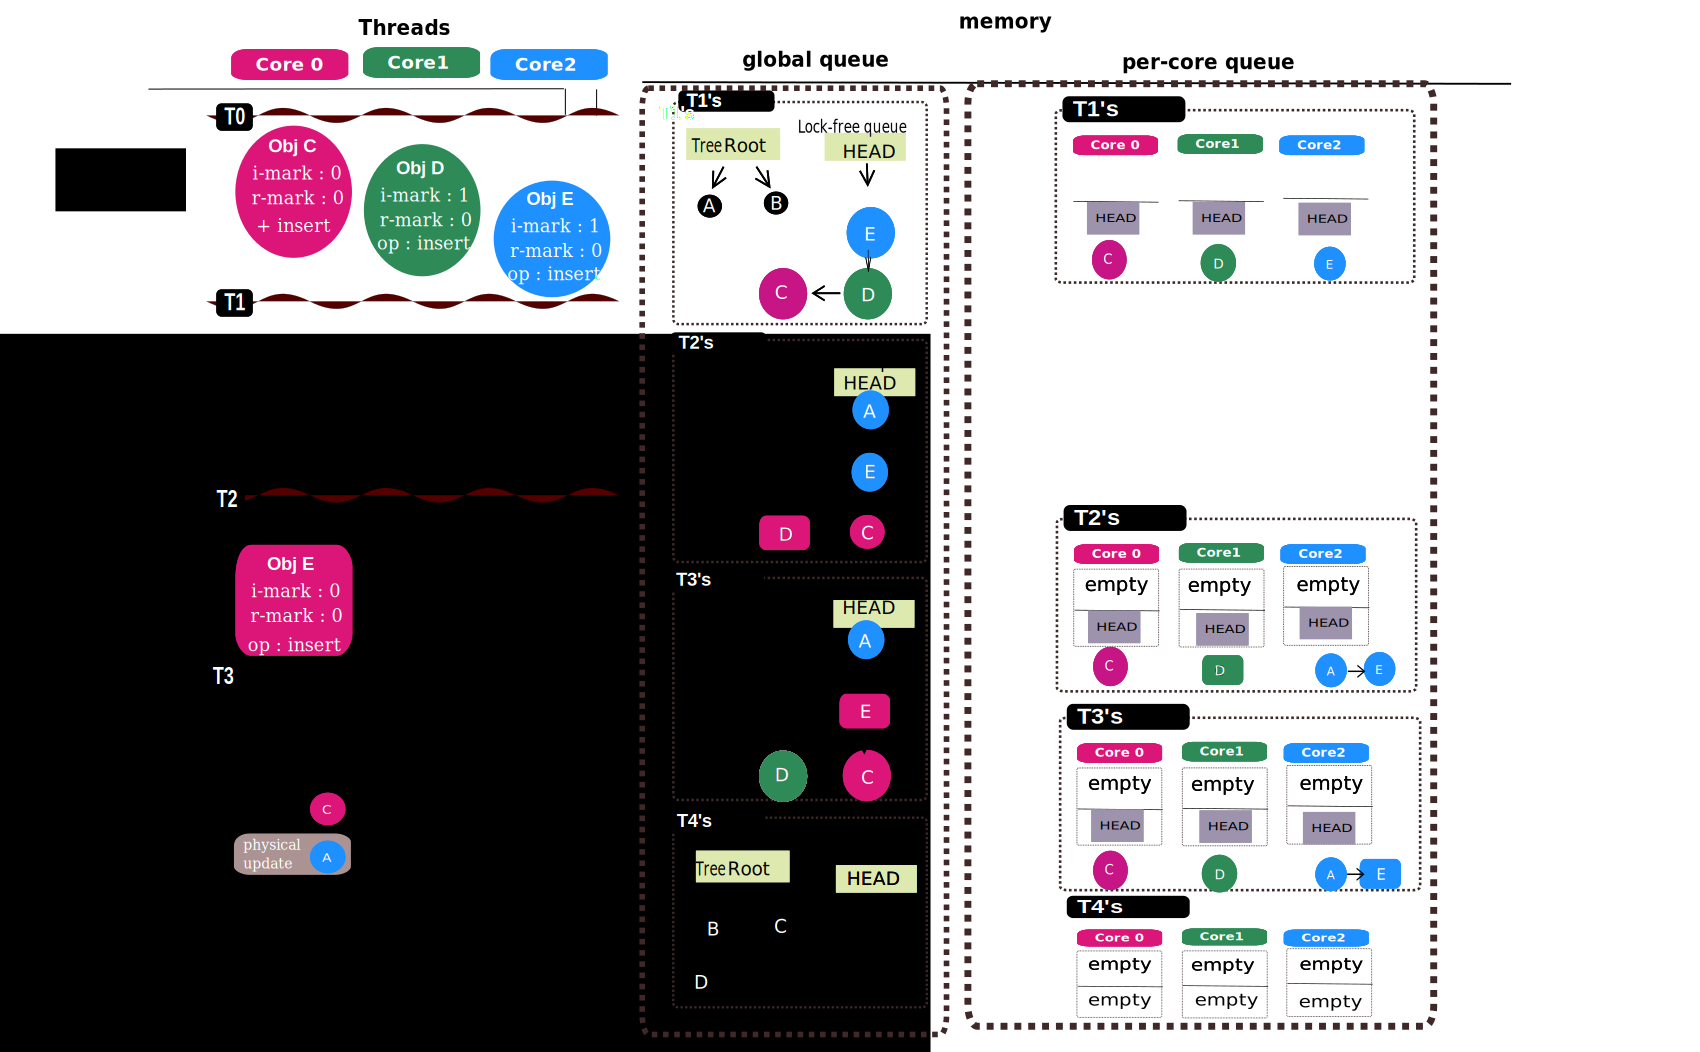
\includegraphics[width=0.8\textwidth,height=0.4\textheight,keepaspectratio]{fig/basic_gldu}
  \end{center}
  \caption{\deferu example showing six update operations and one read
  operation. The execution flows from top to bottom. Memory represents original
  data structure and logging queue at T1, T2 and T3, respectively.}
  \label{fig:basic}
\end{figure*}

\subsection{LDU example}

%$$$$$$$$$$$$$$$$$$$$$$$$$$$$$$$$$$$$$$$$$$$$$$$$$$$$$$$$$$$$$$$$$$$$$$$$$$$$$$$$
%Paragraph 1: Flowchart 그림 설명 
%$$$$$$$$$$$$$$$$$$$$$$$$$$$$$$$$$$$$$$$$$$$$$$$$$$$$$$$$$$$$$$$$$$$$$$$$$$$$$$$$
%


\ifkor
먼저 LDU를 보다 정확하게 설명하기위해, 로그를 global queue 저장한 방법과 per-core queue에 저장한 두가지 방법에 대해서
예를 들어 설명한다. 
그림 \ref{fig:basic} LDU의 하나의 예에 대해서 보여준다. 그림 \ref{fig:basic}은 예로서 queue를 global
queue를 사용하였다. 
7개의 update operation과 1개의 read operation을 LDU에서 어떻게 처리하는지 보여준다.
update operation에 대해서는 앞에서 설명한 심볼을 사용했고 garbage object을 위한 심볼이 추가 되었다.
garbage object는 \res{1}{D}과 같이 rectangle로 표시한다. 
이 그림의 실행 순서는 위에서 부터 아래이다.
그림의 왼쪽은 CPU의 operation 순서를 보여주고 오른쪽은 특정 시간에 메모리에 저장된 자료구조의 내용을 보여준다.
초기 data structure의 트리에는 \inv{0}{A} and \inv{0}{B} 두개의 오브젝트가 들어가고, global
queue에는 아무것도 없다.

그림 \ref{fig:basic}는 시간 순서대로 각단계에 대해서 LDU의 수행 흐름을 보여준다.
먼저 그림에서 concurrent updates 단계에서는 \code{Core0}, \code{Core1} and \code{Core2}가 각각
$\oplus$\inv{1}{C}, $\oplus$\inv{2}{D} and
$\oplus$\inv{3}{E}에 해당하는 3개의 updates oepration을 log로 저장한다. 
Log를 저장하는 queue를 non-blocking queue를 사용하기 때문에, 이 단계에서의 update는 lock이 필요없다. 
즉 모든 thread는 lock에 대한 contention없이 병렬적으로 실행된다. 
\code{T1} 시점이 되면 메모리의 트리는 \inv{0}{A} and \inv{0}{B}의 노드를 가지게 되고, queue에는 
$\oplus$\inv{1}{C}, $\oplus$\inv{2}{D} and $\oplus$\inv{3}{E}가 insert mark 필드가
true로 된 상태로 저장되어 있다. 
update-side absorbing 단계에서는  $\ominus$\inv{1}{D}명령이 수행되면, 새로운 object를 queue에 넣지
않고, mark 필드만 atomic하게 true로 수정한다.  
만약 처음 수행되는 $\ominus$\inv{3}{A} operation이면 queue에 넣는다.
\code{T2} 시점이 되면 메모리의 트리는 변함없고, queue에는 
$\oplus$\inv{1}{C}, $\oplus$\res{2}{D}, $\oplus$\inv{3}{E} and 가
$\ominus$\inv{3}{A} 저장된다. 여기서 \res{2}{D}는 mark필드가 false로 되어 garbage가 된 object이다.
reuse garbage log 단계에서는 \res{2}{D}와 같이 queue에는 들어가 있지만, garbage object인 경우 새롭게
queue에 operation log를 넣지 않고, mark 필드 변경으로 재사용하는 것이다. 
따라서 \res{2}{D}는 \inv{2}{D} 상태로 변경된다. 
\code{T3} 시점이 되면 queue에는 
$\oplus$\inv{1}{C}, $\oplus$\inv{2}{D}, $\oplus$\res{3}{E} and 가
$\ominus$\inv{3}{A} 저장된다.
마지막 단계인 저장된 log를 실행하는 단계에서는 tree에서 사용한 방법으로 lock를 건후 하나의 코어에서 
전체 로그를 update한다. 여기서 garbage log인  $\oplus$\inv{2}{D}을 제외하고 queue에 저장된 순서대로 
$\oplus$\inv{1}{C},$\oplus$\res{3}{E} and 가 $\ominus$\inv{3}{A}의 operation을
수행한다. \code{T4} 시점이 되면 tree에는 
모든 operation이 수행되어, \inv{0}{B}, \inv{0}{C} and \inv{0}{D} 값이 존재하게 된다.
결국 로그를 모두 수행하면 마지막 reader는 같은 tree의 값을 읽게 된다. 

그림 \ref{fig:basicpldu}는 per-core queue에 log를 저장되는 흐름을 설명한다.
global queue와의 차이점만 설명하면,


\else

\fi

\subsection{The LDU Algorithm}
\begin{figure}[tb!]
\inputminted[linenos,fontsize=\footnotesize, tabsize=2]{c}{src/ldu_logical.c}
\rule{\columnwidth}{0.5pt}
\vspace{-\baselineskip}
\caption{\deferu logical update algorithm. \code{logical\_insert} represents
 non-blocking insert function.
It may be called by original insert position without locks. The fastpath is
 that when their object was removed by \code{logical\_remove},
 \code{logical\_insert} just changes node's marking field.}
\label{fig:gldulogicalupdate}
\end{figure}

\subsubsection{logical update: inserting logs}
%$$$$$$$$$$$$$$$$$$$$$$$$$$$$$$$$$$$$$$$$$$$$$$$$$$$$$$$$$$$$$$$$$$$$$$$$$$$$$$$$
%Paragraph 1:LDU Concurrent Updates 알고리즘 코드 및 설명 
%$$$$$$$$$$$$$$$$$$$$$$$$$$$$$$$$$$$$$$$$$$$$$$$$$$$$$$$$$$$$$$$$$$$$$$$$$$$$$$$$
\ifkor

그림 \ref{fig:gldulogicalupdate}는 concurrent updates를 수행하는 코드와 앞에서 설명한 update-side
absorbing logs와 reuse garbage logs에 대한 코드이다. \code{logical\_insert}과
\code{logical\_remove}의 코드에서 가장 먼저하는 것은 이미 update operation이 수행되어 log가 queue에 들어
있는지에 대해서 체크를 한다. 이것은 update함수가 수행하는 도중 어느때나 log를 flush하는 \code{synchronize} 함수가
수행 될 수 있기 때문에, \code{xchg} 함수를 통해 atomic하게 체크를 한다. 또한 \code{xchg}를 통해 old mark
필드가 true라면 이미 queue에 log가 있다는 뜻이므로, atomic하게 false로 수정을 한다.
이것은 앞에서 설명한 update-side absorbing log 기능이며, 1개의 atomic operation으로 update를 수행할 수
있다.
만약 mark 필드카 체크되지 않았다면, 두번째로 queue에 존재하는 로그인지 체크를 한 후, 존재하는 로그라면
이미 앞에서 mark필드를 설정하여 이미 로그를 재활용했으므로 queue에 로그를 넣지 않는다.
만약 처음 사용된 log라면 non-blocking queue에 넣는다.
이 코드는 항상 옳게 동작한다.  
그 이유는 리눅스 update operation이 항상 insert-remove 순서나 remove-insert 순서로 실행되기 때문이다.
%만약 순서가 insert-insert 또는 remove-remove로 동작하면 
\else

\fi


\subsubsection{physical update: applying logs}


\begin{figure}[tb!]
\inputminted[linenos,fontsize=\footnotesize, tabsize=2]{c}{src/ldu_physical.c}
\rule{\columnwidth}{0.5pt}
\vspace{-\baselineskip}
\caption{\deferu physical update algorithm. \code{synchronize\_ldu} may be
 called by reader and converts update log to original data structure
 traversing the lock-less list.}
\label{fig:glduphysicalupdate}
\end{figure}
%$$$$$$$$$$$$$$$$$$$$$$$$$$$$$$$$$$$$$$$$$$$$$$$$$$$$$$$$$$$$$$$$$$$$$$$$$$$$$$$$
%Paragraph 2:LDU Deferred Updates 알고리즘 코드 및 설명 
%$$$$$$$$$$$$$$$$$$$$$$$$$$$$$$$$$$$$$$$$$$$$$$$$$$$$$$$$$$$$$$$$$$$$$$$$$$$$$$$$

\ifkor
그림 \ref{fig:glduphysicalupdate}는 concurrent updates를 통해 저장된 log들을 적용하는 deferred
update 함수에 대한 코드이다.
\code{synchronize\_ldu}는 마치 CoW 처럼 read 전에 호출되기도 하지만, 로그가 쌓이는것을 방지하기 위해 주기적으로
호출되어 로그를 비워준다.
이 함수는 항상 object의 lock이 걸린 상황에서 수행된다. 
LDU는 single consumer가 독점적으로 log를 처리한다.
따라서 제일 먼저 하는일은 queue에 저장된 log를 얻기 위해 atomic xchg operation으로 log의 head 포인터를
얻는다.
그리고 이 순간 부터는 single consumer가 독점적으로 log를 처리하게 된다.
LDU는 주기적으로 log를 비워줘야 하므로, update operation이 수행되는 도중에도 \code{synchronize\_ldu}가
호출될 수 있다.
따라서 항상 origianl data structure에 적용하기 전에 mark 필드를 초기화해야한다.
또한 log를 사용했으면, used 비트를 초기화 하여 해당 log가 queue 없음을 표시한다.
하지만 mark 필드 초기화 과정과 used 비트를 초기화 하는 과정에서, reuse garbase logs 기능 때문에,
언제든지 다시 concurrent updates operation을 통해 mark 필드가 설정될 수 있다.
따라서 한번 더 mark 필드를 체크하여 log를 비워준다.
\else

\fi

\subsubsection{LDU queues}
\begin{figure}[tb!]
\inputminted[linenos,fontsize=\footnotesize, tabsize=2]{c}{src/ldu_queue.c}
\rule{\columnwidth}{0.5pt}
\vspace{-\baselineskip}
\caption{\deferu physical update algorithm. \code{synchronize\_ldu} may be
 called by reader and converts update log to original data structure
 traversing the lock-less list.}
\label{fig:lduqueue}
\end{figure}

\ifkor
LDU의 로그를 저장하기 위한 2가지 queue에 대한 코드는 그림 \ref{fig:lduqueue}와 같다. 
앞에서 설명했듯이 LDU는 어떤 queue를 사용해도 문제 없도록 설계하였다.
따라서 queue 대한 의존성이 없다.
global queue를 사용할 경우 LDU는 항상 head의 first 포인터에 CAS연산으로 성공할 때까지 반복 수행 후 데이터를 넣는다. 
per-core queue를 사용할 경우는 per-core의 hash 테이블을 가지고 온 후 hash 테이블이 넣으려는 log의
data structure와 같은지 체크하고, 다르면 해당 코어에 저장된 log를 lock과 함께 update를 수행한다.
전체 코어의 log를 flush할 필요없이 해당 코어에 저장된 log만 flush하면 되는 이유는 이미 update-side absorbing에
의해 time-sencitive한 operation이 삭제되었기 때문이다.

\else

\fi




%$$$$$$$$$$$$$$$$$$$$$$$$$$$$$$$$$$$$$$$$$$$$$$$$$$$$$$$$$$$$$$$$$$$$$$$$$$$$$$$$
%Reference Sentence 1
%$$$$$$$$$$$$$$$$$$$$$$$$$$$$$$$$$$$$$$$$$$$$$$$$$$$$$$$$$$$$$$$$$$$$$$$$$$$$$$$$

\ifkor
\else
* By default OpLog executes logged updates in temporal order. For example,
consider a linked list. If a process logs an insert operation on one core,
migrates to another core, and logs a remove operation, the remove should
eventually execute after the insert.
* OpLog relies on timestamps from a system-wide synchronized clock to tell it
how to order entries in different cores' log.
*This ordering ensures linearizaility, making OpLog compatible with existing
data structure semantics.
\fi



%$$$$$$$$$$$$$$$$$$$$$$$$$$$$$$$$$$$$$$$$$$$$$$$$$$$$$$$$$$$$$$$$$$$$$$$$$$$$$$$$
%Reference Sentence 1
%$$$$$$$$$$$$$$$$$$$$$$$$$$$$$$$$$$$$$$$$$$$$$$$$$$$$$$$$$$$$$$$$$$$$$$$$$$$$$$$$

%To keep the log from growing without end, we can at any point apply in-order a
%subsequence of the operations at the head of the log to the state to derive a
%new state, and remove these operation from the log[EuroSys 2006 PLS].

%High level operations performed on shared data structures can be divided into
%three groups: read-only, write-only, and read-modify-write[PLS].

%Read-only operations do not mutate the data, write-only operations modify the
%data but do not return a result, and read-modify-write operations change shared
%data and return a result that is dependent on the data read[PLS].

%Both suffer from a complete loss of scalability beyond a rather low concurrency
%level, because all threads must succesfully apply a CAS operation to the shared
%head or tail of the queue in order to complete their operation[FC].


%$$$$$$$$$$$$$$$$$$$$$$$$$$$$$$$$$$$$$$$$$$$$$$$$$$$$$$$$$$$$$$$$$$$$$$$$$$$$$$$$
%Reference Sentence 2:LDU paper
%$$$$$$$$$$$$$$$$$$$$$$$$$$$$$$$$$$$$$$$$$$$$$$$$$$$$$$$$$$$$$$$$$$$$$$$$$$$$$$$$

%This section describes the \deferu algorithm, a lightweight concurrent
%update for update-heavy data structures based on deferred updates.
%Challenges to designing a deferred update mechanism includes 
%performing concurrent update with minimal
%cache line transfers allowing parallel updates.
%At each update operation, \deferu records this update
%operation log to lock-less list.
%Before the read operation, \deferu applies the updates log in chronological
%order.
%In order to deferred update, \deferu divide the update operation 
%into \emph{logical update} and
%\emph{physical update}.
%The \emph{logical update} inserts logs into the lock-less list and carries out
%update side absorbing; on the other hand, the \emph{physical update} executes
%these operations that are minimized by the update side absorbing.

%\begin{figure}[tb]
%  \begin{center}
    %
    % \includegraphics[width=0.5\textwidth,height=0.5\textheight,keepaspectratio]{fig/basic}
%  \end{center}
%  \caption{\deferu example showing six update operations and one read
%  operation. The execution flows from top to bottom. Memory represents original
%  data structure and logging queue at T1, T2 and T3, respectively.}
%  \label{fig:basic}
%\end{figure}

%\subsection{Approach}

%\deferu's scheme for concurrent update is proposed to overcome limitations
%of Linux kernel where 
%both insert and remove operations must not be invoked concurrently for the same
% object, but reads can be concurrently invoked with update.
%\deferu borrows ideas from Oplog's deferred processing and Harris' marking
% scheme.
%The reason is that Linux kernel's object management scheme differs from
% research-oriented data structure such as the lock-free and wait-free data
% structures~\cite{Harris2001Lockfree}~\cite{Fomitchev2004Lockfree}~\cite{Timnat2012}.
%For example, consider the Harris linked list, an insert operation inserts an 
%integer key into the data structure, but Linux kernel inserts their object link.
%The Linux kernel's list operations do not depend on key value.
%Furthermore, Harris linked list node's constructor can be invoked
%upon the insert function's scope, but Linux kernel's node is created on outside scope.
%In this regard, if duplicated remove operation occur, the Linux kernel may
%fail because their link pointer had been freed from destructor.
%Therefore, if a operation is an insert operation, the after operation must occurs 
%remove operation with regard to same object;the remove must execute after the 
%insert, or insert must execute after the remove.
%It means that updates such as insert and remove must not concurrently occur at
%the same object, but reads can occur concurrently.
%\deferu scheme inspires by this operation sequence, and inherits ideas
%from Oplog's deferred processing and Harris's marking scheme.

%\deferu's scheme for concurrent update inspires by Linux kernel's operation
%sequence.
%For example, consider a linked list in Linux kernel, if a operation is an insert
%operation, the after operation must occurs remove operation because Linux
%kernel's object management scheme differs from research-oriented data structure
%such as the lock-free and wait-free data
%structures~\cite{Harris2001Lockfree}~\cite{Fomitchev2004Lockfree}.
%Linux kernel's list operations do not depend on key value, but their 
%list operations depend on their object.
%These structure are their node's constructor can be invoked upon the insert
%function's scope, but Linux kernel's node is created on outside scope.
%In this regard, if duplicated remove operation occur, the Linux kernel may
%fail because their link pointer had been freed from destructor.
%Therefore, the remove must execute after the insert, or insert must execute
%after the remove.
%It means that updates such as insert and remove cannot concurrently occur at
%the same object, but reads can occur concurrently.
%\deferu scheme inspires by this operation sequence, and inherits ideas
%from Oplog's deferred processing and Harris's marking scheme.

%One important algorithm in our proposed novel concurrent update scheme is
%update-side absorbing operation that cancels duplicated operations for
% optimizations.
%A new remove operation, for example, may cancel an existing insert operation
%with regard to same object, so reader can eventually reads consistent data.
%Even though the Oplog's absorbing operation is invoked by
%read, \deferu's absorbing operation is fully invoked by update, so read-side
%performance is enhanced.

%The basic principle of update-side absorbing is that update uses atomic 
%marking operation for the object's mark field, which allows previous operation
% to cancel.
%For instance, if a new remove operation occurs after insert operation of the
%same object, \deferu does not store this operation in the lock-less
%list; instead, it changes the insert mark field to zero using the CAS.
%This mark is checked later when reading operation occurs and the operation log 
%maintained in the lock-less list is applied to original data structure
% atomically.
%This action may give effective update;however, the inserted operation log has
% remained in the lock-less list, so \deferu's reader checks the mark field
% when they convert operation log to original data structure atomically.

%figure : basic principle 
%Figure \ref{fig:basic} gives an example of deferred update with six update
%operations and one read operation.
%In this figure, execution flows from top to bottom.
%The data structure for \emph{physical update} is a tree, and initial values in
%the tree are node \code{A} and \code{B}.
%In contrast, the data structure for \emph{logical update} is lock-less list.
%In the top figure, \code{Core0}, \code{Core1} and \code{Core2} perform the
%logical insert operation to nodes \code{C}, \code{D} and \code{E},
% respectively.
%The logical inserts set the insert mark, and they then insert their
%nodes into lock-less list.
%In this case, none of the lock is needed because \deferu uses the lock-less
%list;all threads can execute the update concurrently.
%At \code{T1}, the tree contains node \code{A}
%and \code{B} and 
%the lock-less list contains node \code{E}, \code{D} and \code{C}.
%When removing the node \code{C}, the node \code{C}, whose mark field was marked
%by insert, atomically cleans up the insert marked field.
%At \code{T2}, the lock-less list contains nodes
%\code{A}, \code{E}, \code{D}, and \code{C}, and the marking field is zero for 
%nodes \code{E} and \code{C}.
%Before running the \code{synchronize} function, they need to lock the original
% tree's lock using the exclusive lock in order to protect the tree's
% operation.
%The \code{synchronize} migrates from lock-less list node to tree node, each of 
%which is the marked node, so nodes \code{A} and \code{D} are migrated.
%Finally, the tree contains nodes \code{D} and \code{B}, so the reader can read
% eventually consistent data.

%First, removing the cancelable operation at update point, \deferu uses the
% update side absorbing instead of read before absorbing.
%Therefore, read before operations in \deferu are fast because read-side
%absorbing operation is eliminated. 
%One notable difference between Oplog and \deferu is that 
%\deferu uses a light weight global queue with non-blocking synchronization 
%for update logs and eliminates time stamps while Oplog is dependent on 
%per-core logs with time stamps.
%By eliminating the global time stamps(hardware-dependent feature), \deferu is
% not dependent on hardware feature.
%Furthermore, update operations in \deferu are also fast because they use
%efficient update-side absorbing that eliminates traversal finding the
%cancelable operation.
%Furthermore, to optimize the log management and minimize the traversal
% overheads during reading, \deferu applies efficient update-side absorbing
% algorithm instead of read-side absorbing algorithm.

%\subsection{logical update}
%\begin{figure}[tb]
%\begin{obeylines}
%\begin{obeyspaces}
%function \(logical\_insert(obj, root) \):
%~~~If CAS(obj.del\_node.mark, 1, 0) $\ne$ 1:  
%~~~    obj.add\_node.mark $\gets$ 1
%~~~    If test\_and\_set\_bit(OP\_INSERT, obj.exist) $\ne$ true:
%~~~        set\_bit(OP\_INSERT, obj.used):
%~~~        obj.add\_node.op $\gets$ OP\_INSERT
%~~~        obj.add\_node.key $\gets$ obj
%~~~        obj.add\_node.root $\gets$ root
%~~~        add\_lock\_less\_list(obj.add\_node)
%~~~
%~~~
%function \(logical\_remove(obj, root) \):
%~~~If CAS(obj.add\_node.mark, 1, 0) $\ne$ 1:  
%~~~    obj.del\_node.mark $\gets$ 1 
%~~~    If test\_and\_set\_bit(OP\_REMOVE, obj.exist) $\ne$ true:
%~~~        set\_bit(OP\_REMOVE, obj.used):
%~~~        obj.del\_node.op $\gets$ OP\_REMOVE
%~~~        obj.del\_node.key $\gets$ obj
%~~~        obj.del\_node.root $\gets$ root
%~~~        add\_lock\_less\_list(obj.del\_node)

%\end{obeyspaces}
%\end{obeylines}
%\rule{\columnwidth}{0.5pt}
%\vspace{-\baselineskip}
%\caption{\deferu logical update algorithm. \code{logical\_insert} represents
% non-blocking insert function.
%It may be called by original insert position without locks. The fastpath is
% that when their object was removed by \code{logical\_remove},
% \code{logical\_insert} just changes node's marking field.}
%\label{fig:logicalupdate}
%\end{figure}

%The pseudo code for \deferu's \emph{logical update} is given in
%figure~\ref{fig:logicalupdate}.
%The \code{logical\_insert}, the concurrent update function, checks whether this
%object already has been removed by \code{logical\_remove}.
%If this object has been removed, \code{logical\_insert} initializes the marking
% field and then they return, which is fastpath.
%The marking field needs synchronization because this field in the
%\emph{logical update} is shared with the \emph{physical update}, so the CAS
% operation is needed.
%When the marking field has been initialized, they set the
%marking field, then they check whether or not this node already has been
% inserted in lock-less list.
%If the node does not exist in lock-less list, then they insert the node into
%lock-less list.

%\subsection{Physical update}
%\begin{figure}[tb]
%\begin{obeylines}
%\begin{obeyspaces}
%function \(synchronize\_ldu(obj, head) \):
%~~~If (head.first = NULL): 
%~~~    return; 
%~~~entry $\gets$ xchg(head.first, NULL);
%~~~for each list node:
%~~~    obj $\gets$ node.key
%~~~    clear\_bit(node.op, obj.exist)
%~~~    If CAS(node.mark, 1, 0) = 1:
%~~~         physical\_update(node.op, obj, node.root)
%~~~    clear\_bit(node.op, obj.used)
%~~~
%function \(physical\_update(op, obj, root) \):
%~~~If op = OP\_INSERT :  
%~~~    call real insert function(obj, root) 
%~~~Else If op = OP\_REMOVE :  
%~~~    call real remove function(obj, root) 

%\end{obeyspaces}
%\end{obeylines}
%\rule{\columnwidth}{0.5pt}
%\vspace{-\baselineskip}
%\caption{\deferu physical update algorithm. \code{synchronize\_ldu} may be
% called by reader and converts update log to original data structure
% traversing the lock-less list.}
%\label{fig:physicalupdate}
%\end{figure}

%The pseudo code for \deferu's \emph{physical update} is given in
%Figure~\ref{fig:physicalupdate}.
%First, they check whether lock-less list is an empty list or not, then they
%iterate the lock-less list.
%If the marking field has been set, they execute migration from
%lock-less to original data structure.
%Because the marking field in \emph{physical update} is shared with
% \emph{logical update}, the CAS operation is needed.
%They initialize the used field, which needs to protect the object from freed
% through destructor.
%The programmer must acquire locks on the \code{synchronize\_ldu} function,
%which migrates log to original data structure.
%Finally, the \code{physical\_update} executes original functions by using the
%operation log.

\newpage
\section{리눅스 커널에 적용}
\label{sec:linux}

%\subsection{Reverse mapping}

%$$$$$$$$$$$$$$$$$$$$$$$$$$$$$$$$$$$$$$$$$$$$$$$$$$$$$$$$$$$$$$$$$$$$$$$$$$$$$$$$
%Paragraph 1: Linux의 reverse mapping에 대한 자세한 설명 
%$$$$$$$$$$$$$$$$$$$$$$$$$$$$$$$$$$$$$$$$$$$$$$$$$$$$$$$$$$$$$$$$$$$$$$$$$$$$$$$$

%This section shows how to apply the \LDU to the complex Linux
%virtual memory system 
이번 장은 리눅스 커널의 업데이트 직렬화에 대한 문제를 풀기 위해,
우리가 어떻게 LUD를 복잡한 리눅스 가상 메모리 시스템에 적용했는지에 대해 설명한다.
이번 장은 더욱 현실적인 내용을 다룬다.
%to solve the update serialization problem;it deals with more practical one.

%The Linux reverse page mapping(rmap), a kernel memory management mechanism,
% consists of anonymous rmap and file rmap, are a update-heavy data structure.
리눅스 역 매핑(rmap)은 커널 메모리 관리 메커니즘(mechanism) 중 하나 이다.
이것은 익명 역 매핑과 파일 역 매핑으로 구성되며 이것은 업데이트 비율이 높은 자료구조이다.
%These two rmaps maintain virtual address(VMAs) to translate physical
%addresses to virtual address~\cite{Dave2004OLSRMAP}, and the rmaps are a shared
% global resource between processes.
이러한 두 가지 rmap은 리눅스의 가상 주소(VMAs)를 관리하고, 이것은 물지 주소(physical address)를 
가상 주소로 변환하는 일을 하며, rmap은 프로세스 간 공유하는 전역 자원(global resource)이다.
%These global resource of rmap are managed by using a interval tree.
이러한 전역 자원인 rmap은 인터벌 트리(interval tree)에 의해 관리된다.
 %To protect these shared tree, Linux kernel uses the reader-writer semaphore,
 %and simultaneous creation of many processes becomes bottlenecks because not
 %only the rmap's update operations can not run in parallel but also update's
%lock brings about the cache invalidation traffic.
이러한 공유 자원을 보호하기 위해, 리눅스는 읽기-쓰리 세마포어(reader-writer semaphore)를 이용하고, 
동시적으로 많은 프로세스가 생성되면 이것은 결국 병목 현상으로 된다. 
그 이유는 rmap의 업데이트 명령어들이 병렬로 실행되지 못할 뿐만 아니라 락 자체가 캐시
커뮤니케이션 오버헤드를 가져오기 때문이다.

%On the contrary, the rmap rarely reads the interval tree when it swaps a
% physical page out to disk, migrates other cpu, or truncates a file.
이와 반대로, ramp은 물리 페이지(physical page)가 디스크로 옮겨 질 때와 다른 CPU로 옮겨질 때 그리고 
파일 사이즈를 줄일 때 간혈 적으로 인터벌 트리를 읽는다.
%In brief, the Linux rmaps are a update-heavy data structure. 

\subsection{익명 역 매핑}


%$$$$$$$$$$$$$$$$$$$$$$$$$$$$$$$$$$$$$$$$$$$$$$$$$$$$$$$$$$$$$$$$$$$$$$$$$$$$$$$$
%Paragraph 1: linux의 anon vma의 공유된 구조에 대한 설명
%$$$$$$$$$$$$$$$$$$$$$$$$$$$$$$$$$$$$$$$$$$$$$$$$$$$$$$$$$$$$$$$$$$$$$$$$$$$$$$$$
%Figure \ref{fig:anonvmaramp} shows the anonymous rmap data structure.
그림 \ref{fig:anonvmaramp}은 익명 rmap에 대한 자료구조를 보여준다.
%When a process spawns, the parent's anonymous vma chain(AVC) are copied
%to a child, and then a new anonymous vma(\code{struct anon\_vma}) is created.
프로세스가 자식을 만들 때, 부모의 익명 메모리 체인(AVC)는 자식에게 복사한다. 
그리고 새로운 익명 가상메모리(\code{struct anon\_vma})는 생성이 된다.
%, indicating the child's AVCs, 
%When a process simultaneously spawns, the more complex
%anonymous rmap data structures are created;the anonymous ramp is one of the
% complex data structure in Linux kernel~\cite{CorbetLWNANON}.
프로세스가 동시적으로 자식 프로세스를 만들 때, 더 복잡한 익명 ramp의 자료구조는 생성된다.
또한 익명 rmap은 리눅스 커널에서 복잡한 자료구조 중 하나이다~\cite{CorbetLWNANON}.
%The anonymous rmap uses the root lock since the AVCs are shared with child
%processes, so this root lock causes a lock contention
%problem~\cite{Andi2011adding}.
익명 ramp은 자식 프로세스간 AVCs를 공유하기 때문에 루트(root)의 락을 사용한다.
따라서 이러한 루트 락은 락 경합 문제를 일으킨다~\cite{Andi2011adding}.  


\begin{figure}[tb]
  \begin{center}
     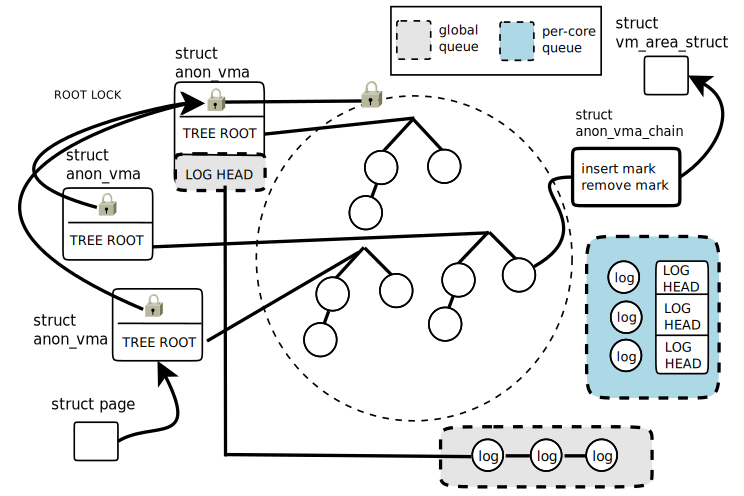
\includegraphics[width=1\textwidth,height=1\textheight,keepaspectratio]{fig/anon_vma}
  \end{center}
  \caption{리눅스 익명 역 매핑에 LDU를 적용한 그림.}
  \label{fig:anonvmaramp}
\end{figure}

%$$$$$$$$$$$$$$$$$$$$$$$$$$$$$$$$$$$$$$$$$$$$$$$$$$$$$$$$$$$$$$$$$$$$$$$$$$$$$$$$
%Paragraph 2: anon vma에 ldu 적용한 방법에 대한 설명 
%$$$$$$$$$$$$$$$$$$$$$$$$$$$$$$$$$$$$$$$$$$$$$$$$$$$$$$$$$$$$$$$$$$$$$$$$$$$$$$$$
%To eliminate this lock contention problem, we add the insert and
%remove mark field in the individual object(\code{struct anon\_vma}),
%and then we implement the update-side removing logs scheme.
락 경합에 대한 문제점을 제거하기 위해서, 우리는 개별적인 오브젝트(\code{struct anon\_vma})에 
삽입과 삭제에 대한 마크 필드를 추가하였다. 
그리고 우리는 업데이트 측면에서 지우는 기술을 구현하였다.
%Understanding the log's position of queue header is important.
로그 큐 헤더에 대한 위치를 이해하는것은 중요하다.
%As noted earlier, since the anonymous rmap uses the root lock, the per-core
% queue version of the LDU logs into a per-core memory with root information, or the global
%queue logs into a root data structure(\code{struct anon\_vma}).
앞에서 설명한봐와 같이, 익명 rmap은 루트의 락을 사용하기 때문에, 퍼코어 큐 버전의 LDU는 
퍼코어 메모리에 루트의 정보와 함께 저장하거나, 글로벌 큐의 경우에는 루트 자료구조((\code{struct anon\_vma}))
에 저장한다. 
%Consequently, the \LDU does not largely modify the original data
%structure, which shows why the \LDU is a lightweight method.
결론적으로, LDU는 원본 자료구조를 많이 수정하지 않는다. 이것은 LDU가 왜 가벼운 방법인지에 
대해서 보여준다.

\subsection{파일 역 매핑}

\begin{figure}[tb]
  \begin{center}
     \includegraphics[width=1\textwidth,height=1\textheight,keepaspectratio]{fig/file_rmap}
  \end{center}
  \caption{리눅스 파일 역 매핑에 LDU를 적용한 그림.}
  \label{fig:fileramp}
\end{figure}

%$$$$$$$$$$$$$$$$$$$$$$$$$$$$$$$$$$$$$$$$$$$$$$$$$$$$$$$$$$$$$$$$$$$$$$$$$$$$$$$$
%Paragraph 1: linux의 file mapped page reverse mapping의 구조에 대한 설명
%$$$$$$$$$$$$$$$$$$$$$$$$$$$$$$$$$$$$$$$$$$$$$$$$$$$$$$$$$$$$$$$$$$$$$$$$$$$$$$$$
%Figure \ref{fig:fileramp} shows the rmap for file.
그림 \ref{fig:fileramp}는 파일에 대한 rmap을 보여준다.
%In order to translate physical addresses to virtual address, the
% page(\code{struct page}) indicates the address space object(\code{struct address\_space}), and
%the address space object manages the VMAs by using the
%interval tree.
물리적 주소를 가상 주소로 변경하기 위해서, 페이지는
 address space 오브젝트(\code{struct address\_space})
를 가리키며, address space 오브젝트는 인터벌 트리를 이용하여 VMAs를 관리한다.
%This interval tree is a shared resource between processes.
이러한 인터벌 트리는 프로세스간 공유하는 자원이다. 
%, so Linux kernel uses the reader-writer semaphore to protect the tree.
%Because the system calls such as \code{fork()}, \code{exit()} and
%\code{mmap()} entail concurrent updating VMAs into the shared resource.
\code{fork()} 그리고 \code{exit()}과 같은 시스템 콜은 VMAs에 대해서 동시적 업데이트를 
수반하므로, 프로세스들이 동시에 많은 시스템 콜을 호출할 때, 파일 ramp은 업데이트 명령어 때문에
직렬화가 된다. 
%when the processes simultaneously invoke these system calls, the
%file rmap can be serialized at the update operations.

%$$$$$$$$$$$$$$$$$$$$$$$$$$$$$$$$$$$$$$$$$$$$$$$$$$$$$$$$$$$$$$$$$$$$$$$$$$$$$$$$
%Paragraph 2: file mapping에 ldu 적용한 방법에 대한 설명 
%$$$$$$$$$$$$$$$$$$$$$$$$$$$$$$$$$$$$$$$$$$$$$$$$$$$$$$$$$$$$$$$$$$$$$$$$$$$$$$$$
%The \LDU can easily be applied to the file ramp data structure.
LDU는 파일 rmap 자료구조에 쉽게 적용될 수 있다. 
%For instance, to use the \LDU, a developer adds log's queue header into the
% per-core memory or into the original data structure(\code{struct address\_space}), and
%then adds mark field to the individual object(\code{struct vm\_area\_struct}).
예를 들어, LDU를 사용하기 위해서는 개발자는 로그의 큐 헤더를 퍼코어 메모리에 저장하던지, 아니면 
원본 자료구조(\code{struct address\_space})에 저장하면 된다. 그리고 각각의 오브젝트(\code{struct
vm\_area\_struct})에 마크필드를 추가하면 된다. 

%Then, the developer modifies update function to logging function without a
% lock.
그리고 개발자는 락 없이 업데이트 함수를 로깅 함수로 수정한다.  
%Finally, the developer creates \code{synchronize} function and calls
%the \code{synchronize} function before the read.
마지막으로 개발자는  \code{synchronize} 함수를 만들고, 이것을 리드 전에 호출되도록 수정한다.
%the mark field adds to the individual object(\code{struct
%vm\_area\_struct}), and then the log's queue is added into the per-core
%memory or the global head object(\code{struct address\_space}).

%This figure clearly shows why the \LDU additionally supports the
%global queue because it is a simpler and easier scheme because the log's head
%pointer is located in the interval tree's data structure.
이 그림은 왜 LDU가 추가적으로 전역 큐를 사용하는지를 보여준다. 
이것은 로그의 헤드 포인터가 인터벌 트리의 자료구조에 위치하기 때문이다.
반면에, 퍼코어 큐는 헤드에 대한 메모리의 위치가 다르므로,  
추가적인 퍼코어 큐에 대한 관리 방법이 필요하다. 
%On the other hand, the
%per-core queue may need an additional per-core queue management scheme due
%to the its isolated memory location.



\begin{figure*}[h]
\begin{center}
\inputminted[linenos,fontsize=\footnotesize,
tabsize=4]{c}{src/ldu_queue_global.c}
\end{center}
%\rule{\columnwidth}{0.5pt}
%\vspace{-\baselineskip}
\caption{LDU의 전역 큐.}
\label{fig:glduphysicalupdate}
\end{figure*}

\subsection{자세한 구현 내용}
%$$$$$$$$$$$$$$$$$$$$$$$$$$$$$$$$$$$$$$$$$$$$$$$$$$$$$$$$$$$$$$$$$$$$$$$$$$$$$$$$
%Paragraph 2: per-core queue 구현에 대한 설명 
%$$$$$$$$$$$$$$$$$$$$$$$$$$$$$$$$$$$$$$$$$$$$$$$$$$$$$$$$$$$$$$$$$$$$$$$$$$$$$$$$
%Because the log's head pointer for the per-core queue is
%separated with the original data structure, the implementation of
%per-core queue uses 
%a per-core hash table method that can allow each object to distinguish.
퍼코어 큐를 위한 로그의 헤드 포인트 위치가 큐는 원본 자료구조와 분리 되어 있으므로, 
퍼코어 큐의 구현은 퍼코어 해시 테이블(per-core hash table) 방법을 이용하였다. 이것은
각각의 오브젝트들을 구분 할 수 있게 해준다.
%The per-core hash table implemented as a direct-mapped cache, which one
%bucket only has an object because recently used objects will be in the hash
%table in a way similar to the OpLog's per-core hash table.
퍼코어 해쉬 테이블은 직접 사상 캐시(direct-mapped cache)를 구현하였다. 이것은 하나의
 해시 버켓(bucket)에는 오직 하나의 오브젝트만 존재하는 방법이다.
그 이유는 최근에 사용된 오브젝트가 다시 사용될 활률이 크기 때문이며, 이것은 OpLog의 
퍼코어 해시 테이블 방법과 비슷하다.
%When this hash table is met a hash conflict, the \LDU evicts the object in the
%hash slot.
만약 해쉬 테이블이 충돌을 만나면, LDU는 충돌난 오브젝트를 해쉬 슬롯에서 부터 내보낸다.
%Moreover, this method reduces additional tasks of programmers because it can
%minimize code modifications and does not need an additional lock.
더욱이, 이러한 방법은 프로그래머의 추가적인 작업을 줄인다. 
그 이유는 이것은 코드의 수정을 최소화할 수 있고 추가적인 락이 필요가 없기 때문이다.
%The per-core hash table, however, incurs a hash conflict overhead.
하지만 퍼코어 해시 테이블은 해시 충돌에 따른 오버헤드를 낳는다.
%This method is useful when a number of the root objects are infrequently
% created like the file rmap(\code{struct address\_space}).
이러한 방법은 파일 rmap(\code{struct address\_space})과 같이
 작은 빈도수로 루트 오브젝트가 생성될 때 효율적이다. 
%On the other hand, since the anonymous rmap severely creates many
%root objects(\code{struct anon\_vma}), it causes a hash conflict overhead.
반면에, 익명 ramp은 극심하게 루트 오브젝트((\code{struct anon\_vma})들을 생성하기 때문에, 
이것은 심한 해쉬 충돌 오버헤드를 발생한다. 
%Therefore, in the case of the anonymous ramp, we did not distinguish object
%headers, but it needs additional tasks with global lock.
그러므로, 익명 rmap과 같은 경우에는 우리는 오브젝트의 헤더를 구별하지 않았다. 
그러나 이것은 추가적인 프로그래머의 작업과 전역 락이 필요하다.



\begin{figure}[h!]
\begin{center}
\inputminted[linenos,fontsize=\footnotesize,
tabsize=4]{c}{src/ldu_queue_per_core.c}
\end{center}
%\rule{\columnwidth}{0.5pt}
%\vspace{-\baselineskip}
\caption{LDU의 퍼코어 큐.}
\label{fig:glduphysicalupdate}
\end{figure}





%$$$$$$$$$$$$$$$$$$$$$$$$$$$$$$$$$$$$$$$$$$$$$$$$$$$$$$$$$$$$$$$$$$$$$$$$$$$$$$$$
%Paragraph 1: 커널 버전 및 코드 분량, 테스트에 대한 설명
%$$$$$$$$$$$$$$$$$$$$$$$$$$$$$$$$$$$$$$$$$$$$$$$$$$$$$$$$$$$$$$$$$$$$$$$$$$$$$$$$
%We have implemented the new deferred update algorithm in Linux 4.5-rc6 kernel,
%and our modified Linux is available as open source. 
우리는 새로운 지연 업데이트 알고르즘을 리눅스 4.5-rc6 커널에 구현하였고, 우리의 
수정된 리눅스는 오픈소스로 이용할 수 있다.  
%The version of global queue modified code is xx that less complex, but per-core
%queue the modified code is xx-xx.
%The implementation is stable enough and has passed the testing
%related with virtual memory, scheduler,
%and file in the Linux Test Project~\cite{LTP}.
우리의 구현은 충분히 안정적이며, 리눅스의 테스트 프로젝트(Linux Test Project)~\cite{LTP}
 중에서 가상 메모리, 스케줄러 그리고 파일과 관련된 테스트를 모두 통과하였다. 

\newpage

\section{평가}
\label{sec:evaluation}
\begin{figure}[h!]
  \begin{center}
    \includegraphics[scale=0.8]{fig/xeon}
  \end{center}
  \caption{실험 환경.}
  \label{fig:xeon}
\end{figure}
 
 \begin{figure}[h]
    \centering
    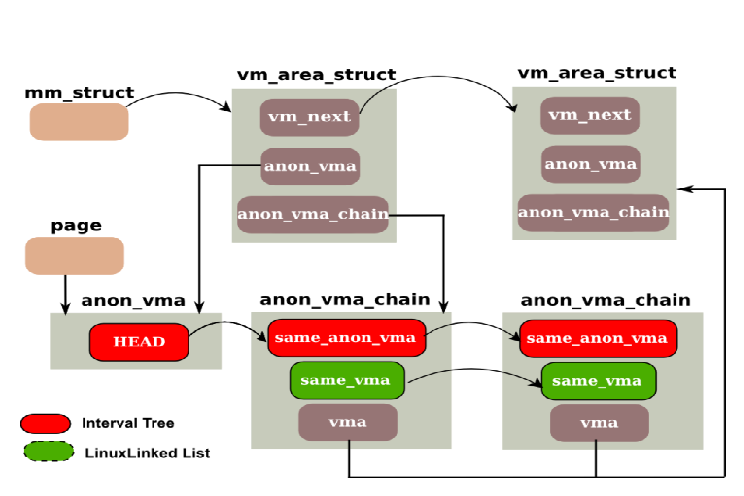
\includegraphics[width=0.8\textwidth]{fig/lockfree}
    \caption{Harris 리스트로 변경하기 전 자료구조}
  \label{fig:lockfree}
\end{figure}
 
 \begin{figure}[h]
    \centering
    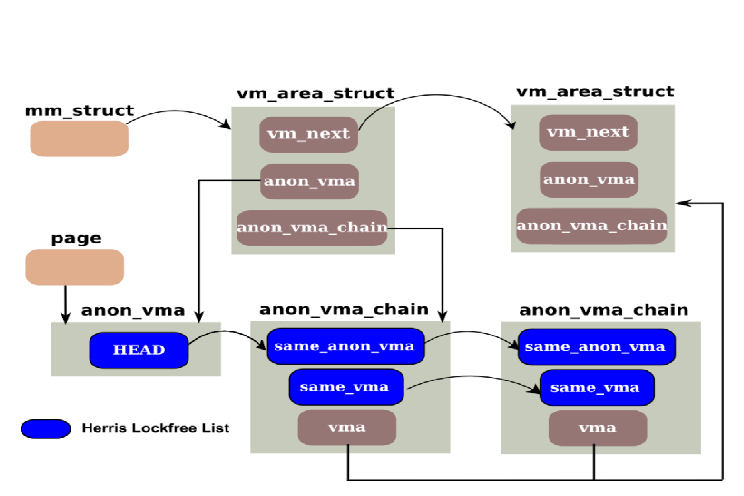
\includegraphics[width=0.8\textwidth]{fig/lockfree_2}
    \caption{Harris 리스트로 변경 후 자료구조}
  \label{fig:lockfree_2}
\end{figure}

\subsection{실험 환경}

%$$$$$$$$$$$$$$$$$$$$$$$$$$$$$$$$$$$$$$$$$$$$$$$$$$$$$$$$$$$$$$$$$$$$$$$$$$$$$$$$
%Paragraph 3: 운영체제 및 커널 버전 설명
%$$$$$$$$$$$$$$$$$$$$$$$$$$$$$$$$$$$$$$$$$$$$$$$$$$$$$$$$$$$$$$$$$$$$$$$$$$$$$$$$
실험을 위해 사용한 하드웨어는 8소켓으로 구성된 120코어 시스템을 사용했으며,
각각의 코어는 인텔 E7-8870 chips(소켓당 15 코어)을 가진다.
메모리는 792기가 바이트 DDR3 DRAM을 사용하였다.
그림~\ref{fig:xeon}은 우리가 사용한 시스템을 보여준다.

%$$$$$$$$$$$$$$$$$$$$$$$$$$$$$$$$$$$$$$$$$$$$$$$$$$$$$$$$$$$$$$$$$$$$$$$$$$$$$$$$
%Paragraph 1: 무엇을 평가 했는지에 대한 설명 
%$$$$$$$$$$$$$$$$$$$$$$$$$$$$$$$$$$$$$$$$$$$$$$$$$$$$$$$$$$$$$$$$$$$$$$$$$$$$$$$$
본 논문에서 제안한 LDU 기법에 대해 평가를 하기 위해, 우리는 리눅스 커널에 LDU를 적용하여 성능을 비교하였다.
비교 대상으로는 수정하지 않은 리눅스 커널과 Harris의 \code{lock-free} 리스트~\cite{Harris2001Lockfree}
알고리즘을 리눅스 커널에 구현하여 추가로 비교 실험을 하였다.
Harris 알고리즘을 사용한 이유는 논블락킹 알고리즘 중에서 대표적인 알고리즘이기 때문이다. 
Harris의 링크드 리스트의 알고리즘은
\textit{sysnchrobench}~\cite{Gramoli2015Synchrobench}와
\textit{ASCYLIB}~\cite{David2015ASYNCHRONIZED}에서 구현된 내용을 이용했으며, Harris 링크드 
리스트를 리눅스 커널에 맞게 수정하여 적용하였다.
Harris 링크드 리스트에 대한 적용을 예를 설명하면, 기존 리눅스는 그림~\ref{fig:lockfree}과 같이 
\code{anon\_vma\_chain}의 내부 변수 중 \code{same\_anon\_vma}는 인터벌 트리로 되어 있고, 
\code{same\_vma}는 리눅스의 링크드 리스트로 되어 있다. 
두 자료구조를 그림~\ref{fig:lockfree_2}와 같이, 
논블락킹 링크드 리스트 중 하나인 Harris 링크드 리스트로 수정하여 구현을 하였다.


%$$$$$$$$$$$$$$$$$$$$$$$$$$$$$$$$$$$$$$$$$$$$$$$$$$$$$$$$$$$$$$$$$$$$$$$$$$$$$$$$
%Paragraph 2-1: Harris Lock free list 구현 내용에 대한 설명 
%$$$$$$$$$$$$$$$$$$$$$$$$$$$$$$$$$$$$$$$$$$$$$$$$$$$$$$$$$$$$$$$$$$$$$$$$$$$$$$$$

%$$$$$$$$$$$$$$$$$$$$$$$$$$$$$$$$$$$$$$$$$$$$$$$$$$$$$$$$$$$$$$$$$$$$$$$$$$$$$$$$
%Paragraph 1: 벤치 마크 대한 설명
%$$$$$$$$$$$$$$$$$$$$$$$$$$$$$$$$$$$$$$$$$$$$$$$$$$$$$$$$$$$$$$$$$$$$$$$$$$$$$$$$
본 연구에서 개발한 LDU는 \code{fork}에 집약적인 응용프로그램과 업데이트 비율이 높은 
자료구조가 효율적인 알고리즘이다. 
따라서, \code{fork}에 집약적인 벤치마크를 선택하였다. 
본 연구에서 선택한 벤치마크 프로그램들은 리눅스의 확장성 벤치마크인 AIM7, 그리고 MOSBENCH에서 
구현된 이메일 서버 벤치마크인 Exim 그리고 마이크로 벤치마크인 Lmbench 이다.
이러한 워크로드들은 모두 역 매핑 때문에 높은 락 경합을 보여준다. 
먼저 AIM7 벤치마크는 리눅스 커뮤니티에서 리눅스 커널에 대한 테스팅 뿐만 아니라 
확장성을 향상 시키기 위해 많이 사용되는 벤치마크이다.
Exim은 실제 사용되고 있는 오픈 소스 응용프로그램이다. 
하지만 이것 역시 리눅스 \code{fork} 때문에 성능에 대한 병목 현상이 발생한다.
마지막으로 마이크로 벤치마크 형식의 \code{fork}에 대한 성능과 확장성에 대해서 보기 위해 
Lmbench를 선택하였다. 

%$$$$$$$$$$$$$$$$$$$$$$$$$$$$$$$$$$$$$$$$$$$$$$$$$$$$$$$$$$$$$$$$$$$$$$$$$$$$$$$$
%Paragraph 2: 비교 대상에 대한 설명
%$$$$$$$$$$$$$$$$$$$$$$$$$$$$$$$$$$$$$$$$$$$$$$$$$$$$$$$$$$$$$$$$$$$$$$$$$$$$$$$$
비교를 위해 4가지 다른 설정으로 실험하였다. 
첫째, 기본 점수를 보기 위해, 수정 없는 리눅스 커널(\code{stock linux})을 사용하였다.
둘째로, 전역 큐 버전의 LDU를 사용해서 실험하였다.  
다음으로, 퍼코어 버전의 LDU를 사용하여 실험하였다. 
마지막으로 앞에서 설명한 Harris의 \code{lock-free} 링크드 리스트를 리눅스 커널을 대상으로 
구현하여 실험하였다.  
%우리는 LDU와 OpLog의 비교는 실제 하드웨어적으로 동기화된 타임스탬프가 존재하지 않는 문제로 
%인해, OpLog와 성능 비교는 수행하지 않았다.

\subsection{AIM7}

\begin{figure}[tb]
  \begin{center}
    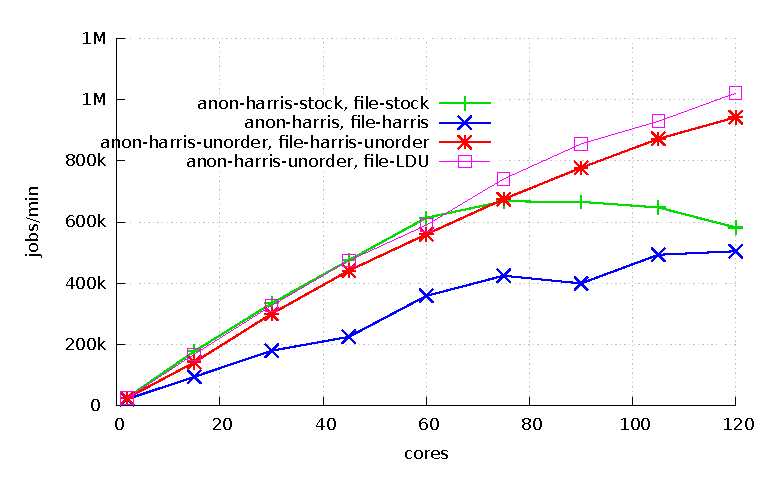
\includegraphics[scale=1]{graph/aim7.eps}
  \end{center}
  \caption{AIM7-multiuser 확장성.}
  \label{fig:aim7}
\end{figure}

\begin{figure*}[tb]
    \centering
    \begin{subfigure}[b]{1\textwidth}
  \begin{center}
        \includegraphics[scale=0.7]{graph/aim7_cpuutils.eps}
  \end{center}
    \end{subfigure}%
    \centering
    \caption{120코어에서 AIM7 CPU 사용량.}
    \label{fig:utilization_aim7}
    
\end{figure*}

\begin{figure*}[tb]
    \centering
    \begin{subfigure}[b]{1\textwidth}
  \begin{center}
        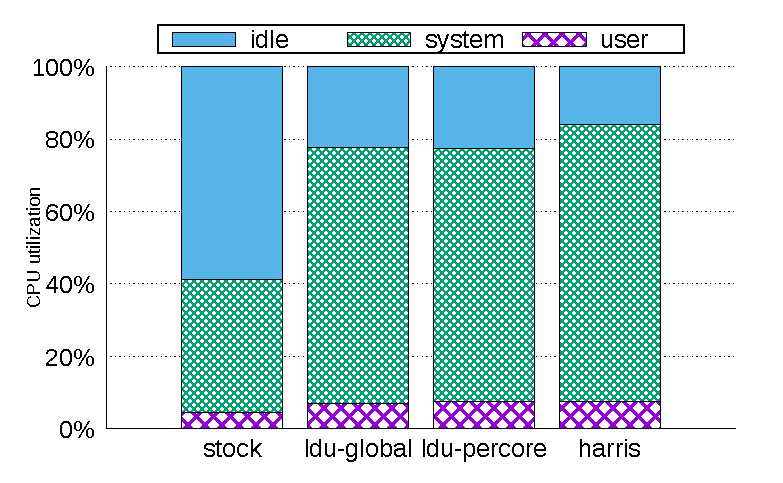
\includegraphics[scale=0.7]{graph/exim_cpuutils.eps}
  \end{center}
    \end{subfigure}
    \centering
    \caption{120코어에서 EXIM CPU 사용량. }
    \label{fig:utilization_exim}
    
\end{figure*}

\begin{figure*}[tb]
    \centering
    \begin{subfigure}[b]{1\textwidth}
  \begin{center}
        \includegraphics[scale=0.7]{graph/lmbench_cpuutils.eps}
  \end{center}
    \end{subfigure}
        \centering
    \caption{120코어에서 Lmbench CPU 사용량.}
    \label{fig:utilization_lmbench}
    
\end{figure*}

%$$$$$$$$$$$$$$$$$$$$$$$$$$$$$$$$$$$$$$$$$$$$$$$$$$$$$$$$$$$$$$$$$$$$$$$$$$$$$$$$
%Paragraph 1: AIM7 실험 결과
%$$$$$$$$$$$$$$$$$$$$$$$$$$$$$$$$$$$$$$$$$$$$$$$$$$$$$$$$$$$$$$$$$$$$$$$$$$$$$$$$


%$$$$$$$$$$$$$$$$$$$$$$$$$$$$$$$$$$$$$$$$$$$$$$$$$$$$$$$$$$$$$$$$$$$$$$$$$$$$$$$$
%Paragraph 1: 워크로드에 대한 설명
%$$$$$$$$$$$$$$$$$$$$$$$$$$$$$$$$$$$$$$$$$$$$$$$$$$$$$$$$$$$$$$$$$$$$$$$$$$$$$$$$
우리는 AIM7-multiuser를 사용하였다. 
이것은 AIM7의 워크로드 중 리눅스 \code{fork}에 집중된 벤치마크이다. 
이러한 multiuser 워크로드는 동시에 많은 프로세스를 생성 한 후 다양한 
일을 수행한다. 
또한 우리는 파일 시스템에 대한 병목현상을 줄이기 위해 리눅스 \code{tmpfs}를 사용하였고, 
코어 수에 비례하여 유져 수를 증가하였다.
 
%$$$$$$$$$$$$$$$$$$$$$$$$$$$$$$$$$$$$$$$$$$$$$$$$$$$$$$$$$$$$$$$$$$$$$$$$$$$$$$$$
%Paragraph 2: 실험 결과에 대한 설명
%$$$$$$$$$$$$$$$$$$$$$$$$$$$$$$$$$$$$$$$$$$$$$$$$$$$$$$$$$$$$$$$$$$$$$$$$$$$$$$$$
AIM7-multiuser에 대한 실험 결과는 그림 ~\ref{fig:aim7}과 같다.
75코어 전 까지는 수정 안한 리눅스는 확장성이 일정하나, 그 이후에는 직렬화된 업데이트 
연산 때문에 병목 현상이 생긴다. 
하지만 120코어까지 Harris 링크드 리스트와 우리의 LDU는 높은 확장성을 가진다.
그 이유는 워크로드들이 업데이트 연산과 읽기-쓰기 세마포어(\code{anon\_vma->rwsem},
\code{mapping->i\_mmap\_rwsem}) 없이 실행될 수 있기 때문이다.
LDU의 퍼코어 큐 버전은 가장 좋은 성능을 보여주고, 확장성도 뛰어나며, 
수정 안 한 리눅스에 비해 1.5배 빠르고 Harris 링크드 리스트보다 1.1배 빠르다.

게다가, 비록 LDU의 전역 큐 버전은 전역 CAS 명령어를 이용하여, 실행되지만, 이 
방법 역시 높은 성능과 확장성을 가진다.
그 이유는 LDU의 최적화 방법 때문에 전역 CAS에 대한 접근이 완화되기 때문이다.
이것은 120코어에서 퍼코어 버전에 비해 2\% 성능 저하가 생긴다. 
더욱이, 수정 안 한 리눅스는 가장 높은 유휴(IDLE) 시간(56\%)을 가진다(그림 ~\ref{fig:utilization_aim7}). 
그 이유는 2가지 세마포어(i.e.,
\code{anon\_vma->rwsem}, \code{mapping->i\_mmap\_rwsem}))를 얻기 위해 스레드가 블락에
걸리기 때문이다.
LDU가 Harris 커널 버전보다 높은 유휴시간을 가지지만, 처리량은 Harris 방법보다 더 높다.
이것은 우리의 LDU 알고리즘이 효율적이라는 것을 보여준다. 

\begin{figure}[tb]
  \begin{center}
    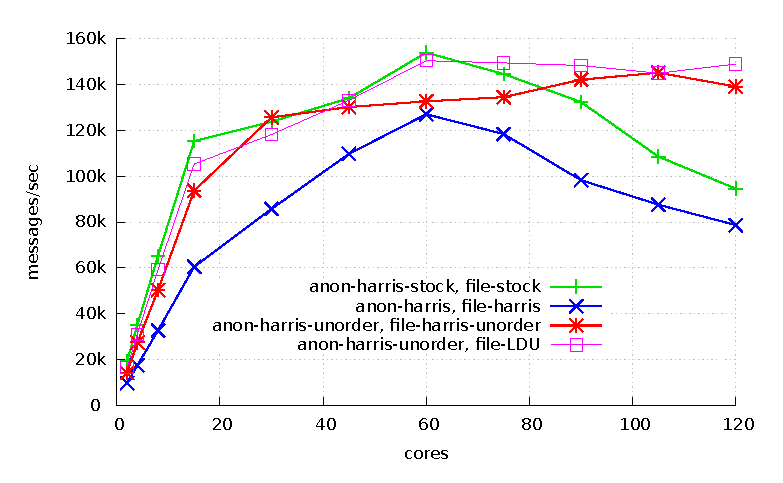
\includegraphics[scale=1]{graph/exim.eps}
  \end{center}
  \caption{Exim 확장성.}
  \label{fig:exim}
\end{figure}

\subsection{Exim}
%$$$$$$$$$$$$$$$$$$$$$$$$$$$$$$$$$$$$$$$$$$$$$$$$$$$$$$$$$$$$$$$$$$$$$$$$$$$$$$$$
%Paragraph 1:  EXIM 실험 결과
%$$$$$$$$$$$$$$$$$$$$$$$$$$$$$$$$$$$$$$$$$$$$$$$$$$$$$$$$$$$$$$$$$$$$$$$$$$$$$$$$

\begin{figure}[tb]
  \begin{center}
    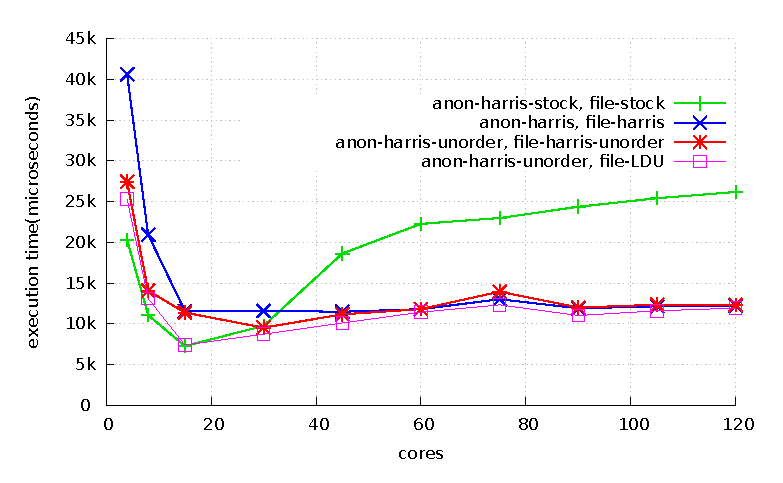
\includegraphics[scale=1]{graph/lmbench.eps}
  \end{center}
  \caption{Lmbench의 프로세스 관리 벤치마크에 대한 실행시간.}
  \label{fig:MicroBench}
\end{figure}

%$$$$$$$$$$$$$$$$$$$$$$$$$$$$$$$$$$$$$$$$$$$$$$$$$$$$$$$$$$$$$$$$$$$$$$$$$$$$$$$$
%Paragraph 1: 워크로드에 대한 설명
%$$$$$$$$$$$$$$$$$$$$$$$$$$$$$$$$$$$$$$$$$$$$$$$$$$$$$$$$$$$$$$$$$$$$$$$$$$$$$$$$
Exim의 성능에 대한 확장성을 측정하기 위하여, 우리는 매니코어 확장성 벤치마크 중 하나인 MOSBENCH를 이용하였다. 
본래 이메일(E-mail) 서버인 Exim의 디자인은 확장성이 있게 설계되었다. 
그 이유는 Exim의 메시지 전달자는 리눅스의 프로세스 기반으로 동작하며, 
여러 프로세스가 병렬적인 방법을 사용하여 메시지를 메일 박스에 전달한다.
이러한 Exim은 \code{fork}가 많이 발생하는 워크로드 중 하나이다. 
클라이언트를 같은 장치에서 실행하였고, 
각각의 클라인언트는 메일 파일에 대한 충돌을 막기 위해, 메시지를 여러 유저에게 보낸다.
Exim은 파일 시스템에서 병목 현상이 발생된다~\cite{SilasBoydWickizer2010LinuxScales48}.
그 이유는 메시지의 바디가 각각의 유저 메일 파일에 추가되기 때문이다.
따라서 우리는 파일 시스템의 병목 지점을 제거하기 위해 분활 된 \textit{tmpfs}를 사용하였다. 

%$$$$$$$$$$$$$$$$$$$$$$$$$$$$$$$$$$$$$$$$$$$$$$$$$$$$$$$$$$$$$$$$$$$$$$$$$$$$$$$$
%Paragraph 2:실험 결과에 대한 설명
%$$$$$$$$$$$$$$$$$$$$$$$$$$$$$$$$$$$$$$$$$$$$$$$$$$$$$$$$$$$$$$$$$$$$$$$$$$$$$$$$
그림~\ref{fig:exim}과 같이 Exim의 결과는 수정안 한 리눅스 커널은 
60코어까지 확장성이 좋게 동작을 한다. 
하지만 60코어 근처부터 확장성이 떨어지는 모습을 볼 수 있다.
45코어 지점에서는 수정 안한 리눅스 커널의 성능이 높게 나오는데, 이것은 LDU의 방법이 
궁극적으로 업데이트 연산을 뒤로 미루는 방법이기 때문에, 락 경합이 덜 발생하면, 오히려 로깅하는 오버헤드 때문에 
성능이 떨어질 수 있다. 
이것은 LDU가 여전히 특정 워크로드와 함께 적은 코어에서의 문제점을 가지고 있다는 것을 보여준다.
하지만 60코어 이후에는 성능이 역전 되어 좋은 성능을 보인다. 

Harris와 LDU는 105코어까지 높은 성능 확장성을 보인다. 
그 이유는 이 두 방법은 세마포어 때문에 기다리는 현상 없이 동시에 업데이트 연산이 가능하기 때문이다. 
LDU의 퍼코어 큐 버전은 더 좋은 성능을 가진다.
그 이유는 이것은 캐시 일관성과 관련한 오버헤드가 없기 때문이며, 120코어에서 수정 안한 
리눅스보다 2.6배 성능 향상을 가지며, Harris 보다 1.2배의 성능 향상을 가진다.
비록 확장성 있는 기술을 적용하였지만, Exim은 105코어부터 성능 확장성에 대해서 문제가 생긴다.
그 이유는 Exim 프로세스들은 상대적으로 큰 크기의 가상 메모리를 사용하기 때문이다.
이것은 결국 프로세스가 종료될 때 가상 메모리에 대한 초기화 오버헤드를 낳으며,
결국 많은 소프트 페이지 폴트(Soft Page Fault)를 야기한다. 
이것은 특히 NUMA 구조와 같은 구조에서는 원격 메모리를 접근하는 현상 때문에 더욱 많은 오버헤드를 야기한다. 
Harris 링크드 리스트는 15\%의 유휴 시간을 가진 반면, 퍼코어 큐 버전의 LDU는 22\%의 유휴 시간을 가진다.
그 이유는 LDU의 효율적인 알고리즘 때문이다(그림~\ref{fig:utilization_exim}).

\subsection{Lmbench}
%$$$$$$$$$$$$$$$$$$$$$$$$$$$$$$$$$$$$$$$$$$$$$$$$$$$$$$$$$$$$$$$$$$$$$$$$$$$$$$$$
%Paragraph 1: %워크로드에 대한 설명
%$$$$$$$$$$$$$$$$$$$$$$$$$$$$$$$$$$$$$$$$$$$$$$$$$$$$$$$$$$$$$$$$$$$$$$$$$$$$$$$$
Lmbench는 다양한 마이크로(Micro) 벤치마크를 포함하고 있다. 
우리는 이러한 다양한 마이크로 벤치마크 중 프로세스 관리에 대한 워크로드를 사용하였다. 
워크로드는 기본적인 프로세스 관리에 대한 프로세스 생성, 
프로그램 시작, 그리고 문맥교환들에 대해서 성능을 측정한다.
그리고 우리는 프로세스 생성에 대한 워크로드에 대해 병렬 옵션 값인 1000을 사용하여 수행하였다. 

%$$$$$$$$$$$$$$$$$$$$$$$$$$$$$$$$$$$$$$$$$$$$$$$$$$$$$$$$$$$$$$$$$$$$$$$$$$$$$$$$
%Paragraph 2: 실험 결과에 대한 설명
%$$$$$$$$$$$$$$$$$$$$$$$$$$$$$$$$$$$$$$$$$$$$$$$$$$$$$$$$$$$$$$$$$$$$$$$$$$$$$$$$
Lmbench의 결과는 그림~\ref{fig:MicroBench}에서 보여주며, 세로축에 대한 결과는 실행 시간이다.
45코어까지, 수정 안 한 리눅스 커널은 일정한 확장성을 보이며, 그 이후 실행시간을 늘어난다.
퍼코어 버전의 LDU는 120코어에서 수정 안 한 리눅스 커널에 2.7배 성능향상으로 보이며, 
Harris 리스트에 비해 1.1배의 성능향상을 보인다.
수정 안 한 리눅스는 69\%의 유휴 시간을 가진 반면 다른 방법들은 약 35\% 정도의 유휴시간을 가진다.
그 이유는 수정 안한 리눅스 커널은 2가지 RMAP 세마포어(\code{anon\_vma->rwsem},
\code{mapping->i\_mmap\_rwsem})(그림~\ref{fig:utilization_lmbench})를 기다리기 때문이다. 
사실, 우리의 LDU의 개발 동기는 120코어에서 성능과 확장성을 개선하는 것이다. 
따라서 우리는 적은 코어(30코어 이내)에서의 성능은 고려하지 않았다.
하지만 30코어까지 우리의 LDU는 수정 안한 리눅스 커널과 비슷한 성능을 보인다. 
반면, Harris 링크드 리스트는 60코어 까지 안 좋은 성능을 보여준다. 
이러한 현상은 LDU가 효율적인 알고리즘 이라는 것을 보여준다.

\subsection{업데이트 비율}

%$$$$$$$$$$$$$$$$$$$$$$$$$$$$$$$$$$$$$$$$$$$$$$$$$$$$$$$$$$$$$$$$$$$$$$$$$$$$$$$$
%Paragraph 2:  실험을 수행한 이유
%$$$$$$$$$$$$$$$$$$$$$$$$$$$$$$$$$$$$$$$$$$$$$$$$$$$$$$$$$$$$$$$$$$$$$$$$$$$$$$$$
본 논문에서 제안하는 LDU는 Update-heavy한 자료구조를 위한 방법이다. 
따라서 리더가 많아질 경우 성능이 떨어지는 단점을 가진다. 
그 이유는 LDU의 읽기 연산은 로그를 적용하는 \code{synchronize} 함수를 호출하므로, 
그 동안 쌓인 로그들을 적용하게 되는데, \code{synchronize} 함수의 
연산 때문에 읽기 연산이 많이 지면 성능이 떨어진다.
따라서, 우리는 어느정도 까지 영향을 미치는지 확인하기 위해, 연산이 자주 발생하는 경우를 
대상으로 실험을 하였다. 

읽기 연산에 대한 효과를 이해하기 위해, 읽기 연산을 업데이트 연산의 비율에 
맞게 추가하여 성능을 측정하는 실험을 하였다.
실험을 단순화 하기 위해 익명 RMAP 자료 구조는 LDU의 전역 큐 버전을 이용하였고, 
파일 RMAP에 대해서는 순차적으로 읽기 연산(\code{lock}, \code{synchronize}) 비율을 증가 시켰다.
예를 들어 99\%는 파일 RMAP에 대해서 업데이트 연산이 99번 수행할 때 1번의 읽기 연산이 
일어나는 것을 의미하고, 순차적으로 90\%는 9번 업데이트에 1번의 읽기 연산을 의미한다.

\begin{figure}[h!]
    \centering
    \begin{subfigure}[b]{1\textwidth}
        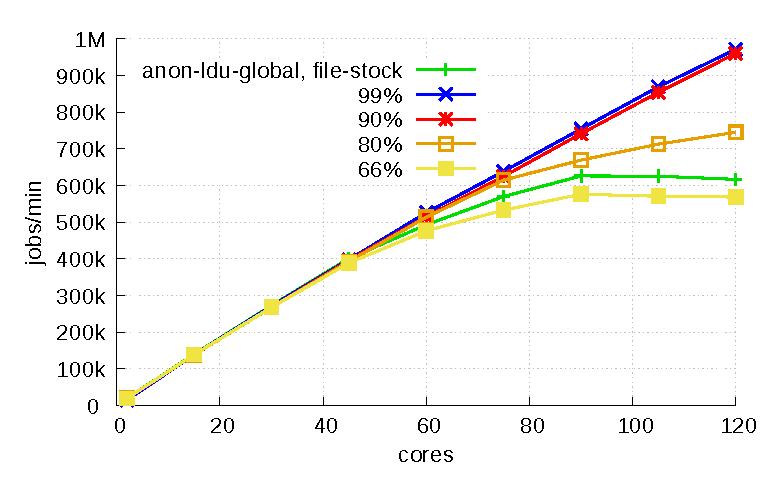
\includegraphics[height=2.5in]{graph/ratio_aim7_core.eps}
    \end{subfigure}%
    \caption{업데이트 비율에 따른 AIM7 확장성.}
    \label{fig:UpdateRate_aim7_2}
\end{figure}
 
 
%$$$$$$$$$$$$$$$$$$$$$$$$$$$$$$$$$$$$$$$$$$$$$$$$$$$$$$$$$$$$$$$$$$$$$$$$$$$$$$$$
%Paragraph 2: 실험 결과에 대한 설명
%$$$$$$$$$$$$$$$$$$$$$$$$$$$$$$$$$$$$$$$$$$$$$$$$$$$$$$$$$$$$$$$$$$$$$$$$$$$$$$$$
그림~\ref{fig:UpdateRate_aim7_2}는 AIM7의 실험 결과를 보여준다.
AIM7의 경우 다른 2가지 벤치마크(Exim, Lmbench)에 비해 덜 \code{fork}에 의존적인 
벤치마크이기 때문에, 읽기 연산이 호출되는 간격이 상대적으로 짧다.
그 결과, 비록 자료구조가 80\%의 업데이트 비율(4개의 업데이트 연산 일때 1개의 읽기 연산을 수행)을 
가지더라도, 수정 안 한 리눅스에 비해 높은 성능을 가진다. 
AIM7의 성능에 대한 확장성은 90\% 이상의 경우 경우 높은 성능 확장성을 가진다.
 
\begin{figure}[h!]
    \centering
    \begin{subfigure}[b]{1\textwidth}
        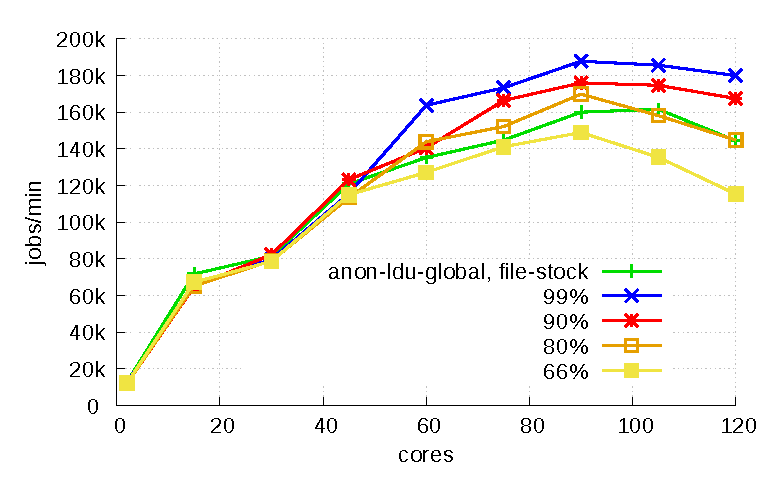
\includegraphics[height=2.5in]{graph/ratio_exim_core.eps}
    \end{subfigure}%
    \caption{업데이트 비율에 따른 Exim 확장성.}
    \label{fig:UpdateRate_exim_2}
\end{figure}


%$$$$$$$$$$$$$$$$$$$$$$$$$$$$$$$$$$$$$$$$$$$$$$$$$$$$$$$$$$$$$$$$$$$$$$$$$$$$$$$$
%Paragraph 2: 실험 결과에 대한 설명
%$$$$$$$$$$$$$$$$$$$$$$$$$$$$$$$$$$$$$$$$$$$$$$$$$$$$$$$$$$$$$$$$$$$$$$$$$$$$$$$$
Exim은 \code{fork}를 많이 호출하는 워크로드 중 하나이다. 
따라서 업데이트 연산이 빨리 호출되는 특징을 가지며, 이것은 읽기 연산의 간격도 짧다는 것을 의미한다.
즉 AIM7과는 다르게 \code{synchronize} 함수가 자주 호출된다는 것을 의미한다.
그 결과, 80\% 이하의 업데이트 연산 비율을 가지면 수정 안 한 리눅스 보다 안 좋은 성능을 가진다.
LDU는 90\% 이상의 업데이트 가질 때 부터 더 높은 성능을 가진다.

\begin{figure}[h!]
    \centering
    \begin{subfigure}[b]{1\textwidth}
        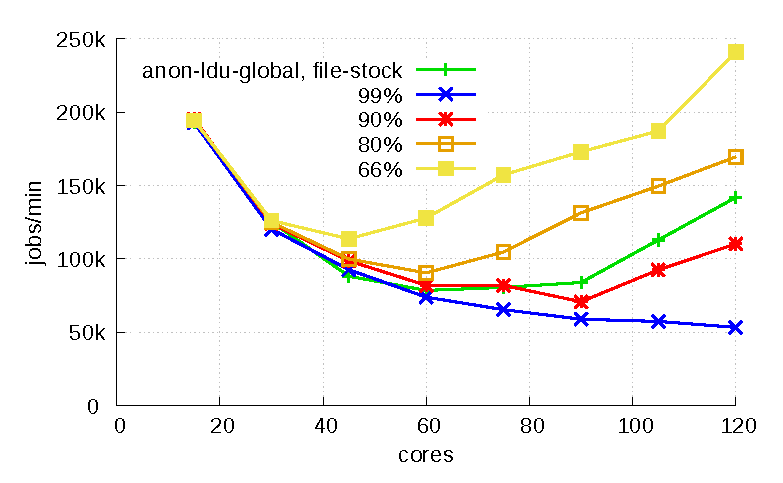
\includegraphics[height=2.5in]{graph/ratio_lmbench_core.eps}
    \end{subfigure}%
    \caption{업데이트 비율에 따른 Lmbench 확장성.}
    \label{fig:UpdateRate_lmbench_2}
\end{figure}

%$$$$$$$$$$$$$$$$$$$$$$$$$$$$$$$$$$$$$$$$$$$$$$$$$$$$$$$$$$$$$$$$$$$$$$$$$$$$$$$$
%Paragraph 2: 실험 결과에 대한 설명
%$$$$$$$$$$$$$$$$$$$$$$$$$$$$$$$$$$$$$$$$$$$$$$$$$$$$$$$$$$$$$$$$$$$$$$$$$$$$$$$$
Lmbench는 Exim과 비슷하게 \code{fork}가 자주 호출 되는 워크로드이다.
Lmbench는 실행 시간을 보여주므로, 낮을 수록 높은 성능을 보여준다. 
실험 결과 Exim과 비슷한 결과를 보이는데, 이것은 수정 안 한 리눅스가 80\%의 업데이트 
비율을 가질 때 더 좋은 성능을 가진다.
하지만 Lmbench는 굉장히 \code{fork}가 자주 호출되는 마이크로 벤치마크이기 때문에 업데이트 연산의 비율이 
90\%가 되면 수정 안한 리눅스 보다는 성능이 좋지만, 확장성이 떨어지는 특징을 가진다.
하지만 LDU는 읽기가 상당히 자주 호출되는 워크로드라도 업데이트 비율이 90\% 이상이면 
높은 성능을 보여준다.
 


\chapter{결론 및 향후 연구}\label{sec:concl}

\section{결론}
%We proposed and evaluated a novel concurrent update method, \LDU, to maximally
%improve the performance scalability of Linux kernel in many core systems. 
우리는 새로운 동시적 업데이트 방법인 LDU를 제안하였고, 평가하였고, 
이것은 매니코어 시스템에서 리눅스 커널의 성능 확장성을 향상시킨다.
%Such improvement was possible through eliminating the  synchronized time-stamp
%counters management overhead found in a previous well-known scheme, OpLog.
우리의 방법은 사전에 연구되어 잘 알려진 로그 기반 알고리즘인 OpLog의 동기화된 타임
 스템프 카운터의 관리에 따른 오버헤드를 제거 할 수 있다. 
%Our experiments using a Linux kernel with our \LDU implementation
%revealed that the proposed \LDU shows better performance up to 2.7 times
%stock Linux kernel on the 120 core machine.
우리의 LDU를 리눅스 커널에 구현하여 수행한 우리의 실험은 기존 리눅스 커널에 비해 120코어 
공유 메모리 기반 컴퓨팅 환경에서 2.7배까지 성능 향상을 이루었다. 
%The \LDU is implemented on to Linux kernel 4.5-rc6 and available as open-source
%from \url{https://github.com/manycore-ldu/ldu}.
우리는 이러한 LDU를 리눅스 커널 4.5-rc6에 구현하였으며, 본 결과물은
아래 사이트에서 오픈소스로 이용할 수 있다.
\begin{center}
\url{https://github.com/manycore-ldu/ldu}
\end{center}

\newpage
\section{향후 연구}
%While the proposed technique achieves significant improvement in performance
%scalability through eliminating time-sensitive logs, there still remain the
%data structures to consider to further improve the scalability (i.e., stack and
%queue data structures).
우리가 제안한 기술은 시간에 예민한 로그를 업데이트 순간 마다 지움으로
 상당한 성능에 대한 향상성을 얻었으나, 이것은 여전히 특정한 자료구조(예를 들어 스택, 큐)
  같은 경우에는 남은 명령어들 마다 시간 순서가 필요하므로 적용하지 못한다.
%Future direction of research is to create a new synchronization scheme by
%combining two techniques(the \LDU and the OpLog) to support the stack and
%queue.
향후 연구로는 LDU의 기술과 OpLog의 기술을 통합하여 스택과 큐를 지원학 위해
 새로운 동기화 기술을 개발하는 것이다. 

%\section{Acknowledgments}
%This work was supported by Institute for Information \& communications
% Technology Promotion (IITP) grant funded by the Korea government (MSIP) (14-824-09-
%011, “Research Project on High Performance and Scalable Manycore Operating
% System”)



%\begin{thebibliography}{1}
%\bibliographystyle{IEEEtran}
\bibliographystyle{plain}
%\bibliography{ref}
\bibliography{ref}
%\end{thebibliography}


\newpage
\addcontentsline{toc}{content}{Abstract}% 목차(TOC)에 추가
\hfill \break

\noindent
\Large{\textbf{Abstract}}

\noindent
\Large{\textbf{A Lightweight Log-based Deferred Update for Linux Kernel
Scalability}}

\normalsize{
\hfill \break
\begin{center}
\raggedleft{\textit{by Kyong, Joohyun}}\\
\raggedleft{\textit{Department of Computer Science}}\\
\raggedleft{\textit{Graduate School, Kookmin University,}}\\
\raggedleft{\textit{Seoul, Korea}}
\end{center}
\hfill \break

In highly parallel computing systems with many-cores, a few critical factors
cause performance bottlenecks severely limiting scalability.
The kernel data structures with high update rate naturally cause performance
bottlenecks due to very frequent locking of the data structures.
There have been research on log-based synchronizations with time-stamps that
have achieved significant level of performance and scalability improvements.
However, sequential merging operations of the logs with time-stamps pose another
sources of scalability degradation.

To overcome the scalability degradation problem, we introduce a lightweight
log-based deferred update method, combining the log-based concepts in the
distributed systems and the minimal hardware-based synchronization in the
shared memory systems.
The main contributions of the proposed method are:(1) we propose a lightweight
log-based deferred update method, which can eliminate synchronized time-stamp
counters that limits the performance scalability;and (2) we implemented the
 proposed method in the Linux 4.5-rc6 kernel for two representative data
 structures (anonymous reverse mapping and file mapping) and evaluated the
performance improvement due to our proposed novel light weight update method.
Our evaluation study showed that application of our method could
achieve from 1.5x through 2.7x performance improvements in 120 core
systems.}

%% 본문 끝
\end{document}
